%%% Hlavní soubor. Zde se definují základní parametry a odkazuje se na ostatní části. %%%

%% Verze pro jednostranný tisk:
% Okraje: levý 40mm, pravý 25mm, horní a dolní 25mm
% (ale pozor, LaTeX si sám přidává 1in)
\documentclass[12pt,a4paper]{report}
\setlength\textwidth{145mm}
\setlength\textheight{247mm}
\setlength\oddsidemargin{15mm}
\setlength\evensidemargin{15mm}
\setlength\topmargin{0mm}
\setlength\headsep{0mm}
\setlength\headheight{0mm}
% \openright zařídí, aby následující text začínal na pravé straně knihy
\let\openright=\clearpage

\renewcommand\baselinestretch{1.3} % riadkovanie jeden a pol

%% Pokud tiskneme oboustranně:
% \documentclass[12pt,a4paper,twoside,openright]{report}
% \setlength\textwidth{145mm}
% \setlength\textheight{247mm}
% \setlength\oddsidemargin{15mm}
% \setlength\evensidemargin{0mm}
% \setlength\topmargin{0mm}
% \setlength\headsep{0mm}
% \setlength\headheight{0mm}
% \let\openright=\cleardoublepage

%% Pokud pouľíváte csLaTeX (doporučeno):
%\usepackage{czech}
%% Pokud nikoliv:
%\usepackage[czech]{babel}
%\usepackage[T1]{fontenc}

%% Pouľité kódování znaků: obvykle latin2, cp1250 nebo utf8:
\usepackage[utf8]{inputenc}
\usepackage[T1]{fontenc}

%% Ostatní balíčky
\usepackage{graphicx}
\usepackage{amsthm}
\usepackage{amssymb}
\usepackage{alltt}
\usepackage{todonotes}
\usepackage{algorithmic}
\usepackage[chapter]{algorithm}
\usepackage{enumerate}
\usepackage{multirow}
\usepackage{threeparttable}
\usepackage{listings}
\usepackage{algorithmic}
\usepackage[chapter]{algorithm}

\usepackage{color}
\definecolor{dkgreen}{rgb}{0,0.6,0}
\definecolor{gray}{rgb}{0.5,0.5,0.5}
\definecolor{mauve}{rgb}{0.58,0,0.82}
\newcommand{\lstfont}{\small\ttfamily}
\lstset{ %
  language=,                % the language of the code
  basicstyle=\lstfont,           % the size of the fonts that are used for the code
  %numbers=left,                   % where to put the line-numbers
  %numberstyle=\tiny\color{gray},  % the style that is used for the line-numbers
  %stepnumber=2,                   % the step between two line-numbers. If it's 1, each line 
                                  % will be numbered
  numbersep=5pt,                  % how far the line-numbers are from the code
  backgroundcolor=\color{white},      % choose the background color. You must add \usepackage{color}
  showspaces=false,               % show spaces adding particular underscores
  showstringspaces=false,         % underline spaces within strings
  showtabs=false,                 % show tabs within strings adding particular underscores
  frame=single,                   % adds a frame around the code
  rulecolor=\color{black},        % if not set, the frame-color may be changed on line-breaks within not-black text (e.g. commens (green here))
  tabsize=2,                      % sets default tabsize to 2 spaces
  captionpos=b,                   % sets the caption-position to bottom
  breaklines=true,                % sets automatic line breaking
  breakatwhitespace=false,        % sets if automatic breaks should only happen at whitespace
  title=\lstname,                   % show the filename of files included with \lstinputlisting;
                                  % also try caption instead of title
  keywordstyle=\color{blue},          % keyword style
  commentstyle=\color{dkgreen},       % comment style
  stringstyle=\color{mauve},         % string literal style
  escapeinside={\%*}{*)},            % if you want to add a comment within your code
  morekeywords={*,...},              % if you want to add more keywords to the set
}

\renewcommand{\algorithmicrequire}{\textbf{Input:}}
\renewcommand{\algorithmicensure}{\textbf{Output:}}

\renewcommand{\algorithmicforall}{\textbf{for each}}

\renewcommand{\algorithmiccomment}[1]{// #1}

% pekne pokope definujeme potrebne udaje
\def\mftitle{Inference of an XML Schema with the Knowledge of XML Operations}
\def\mfthesistype{Master Thesis}
\def\mfauthor{Mário Mikula}
\def\mfadvisor{RNDr. Irena Mlýnková, Ph.D.}
\def\mfplacedate{Praha, 2011}

%% Balíček hyperref, kterým jdou vyrábět klikací odkazy v PDF,
%% ale hlavně ho pouľíváme k uloľení metadat do PDF (včetně obsahu).
%% POZOR, nezapomeňte vyplnit jméno práce a autora.
\usepackage[ps2pdf,unicode]{hyperref}   % Musí být za vąemi ostatními balíčky
\hypersetup{pdftitle=\mftitle}
\hypersetup{pdfauthor=\mfauthor}

%%% Drobné úpravy stylu

% Tato makra přesvědčují mírně oąklivým trikem LaTeX, aby hlavičky kapitol
% sázel příčetněji a nevynechával nad nimi spoustu místa. Směle ignorujte.
%\makeatletter
%\def\@makechapterhead#1{
%  {\parindent \z@ \raggedright \normalfont
%   \Huge\bfseries \thechapter. #1
%   \par\nobreak
%   \vskip 20\p@
%}}
%\def\@makeschapterhead#1{
%  {\parindent \z@ \raggedright \normalfont
%   \Huge\bfseries #1
%   \par\nobreak
%   \vskip 20\p@
%}}
%\makeatother

% Toto makro definuje kapitolu, která není očíslovaná, ale je uvedena v obsahu.
\def\chapwithtoc#1{
\chapter*{#1}
\addcontentsline{toc}{chapter}{#1}
}


% Theorem environment
\newenvironment{definition}[1][Definition]{\begin{trivlist}
\item[\hskip \labelsep {\bfseries #1}]}{\end{trivlist}}


\begin{document}

% Trochu volnějąí nastavení dělení slov, neľ je default.
\lefthyphenmin=2
\righthyphenmin=2

%%% Titulní strana práce

\pagestyle{empty}
\begin{center}

\large

Charles University in Prague

\medskip

Faculty of Mathematics and Physics

\vfill

{\bf\Large \mfthesistype}

\vfill

\centerline{\mbox{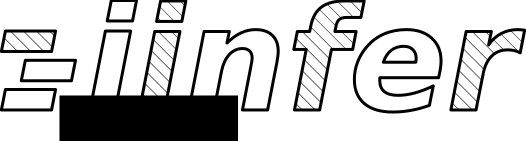
\includegraphics[width=60mm]{logo.eps}}}

\vfill
\vspace{5mm}

{\LARGE \mfauthor}

\vspace{15mm}

% Název práce přesně podle zadání
{\LARGE\bfseries \mftitle}

\vfill

% Název katedry nebo ústavu, kde byla práce oficiálně zadána
% (dle Organizační struktury MFF UK)
Department of Software Engineering

\vfill

\begin{tabular}{rl}

Supervisor of the master thesis: & \mfadvisor \\
\noalign{\vspace{2mm}}
Study programme: & Informatika \\
\noalign{\vspace{2mm}}
Specialization: & ISS \\
\end{tabular}

\vfill

% Zde doplňte rok
\mfplacedate

\end{center}

\newpage

%%% Následuje vevázaný list -- kopie podepsaného "Zadání diplomové práce".
%%% Toto zadání NENÍ součástí elektronické verze práce, nescanovat.

%%% Na tomto místě mohou být napsána případná poděkování (vedoucímu práce,
%%% konzultantovi, tomu, kdo zapůjčil software, literaturu apod.)

\openright

\noindent
I would like to thank my supervisor RNDr. Irena Mlýnková, Ph.D., for her helpful advices, corrections and suggestions.

\newpage

%%% Strana s čestným prohláąením k diplomové práci

\vglue 0pt plus 1fill

\noindent
I declare that I carried out this master thesis independently, and only with the cited
sources, literature and other professional sources.

\medskip\noindent
I understand that my work relates to the rights and obligations under the Act No.
121/2000 Coll., the Copyright Act, as amended, in particular the fact that the Charles
University in Prague has the right to conclude a license agreement on the use of this
work as a school work pursuant to Section 60 paragraph 1 of the Copyright Act.

\vspace{10mm}

\hbox{\hbox to 0.5\hsize{%
In ........ date ............
\hss}\hbox to 0.5\hsize{%
Signature
\hss}}

\vspace{20mm}
\newpage

%%% Povinná informační strana diplomové práce

\vbox to 0.5\vsize{
\setlength\parindent{0mm}
\setlength\parskip{5mm}

Název práce:
Odvozování XML schémy se znalostí XML operací
% přesně dle zadání

Autor:
\mfauthor

Katedra:  % Případně Ústav:
Katedra softwarového inženýrství
% dle Organizační struktury MFF UK

Vedoucí diplomové práce:
\mfadvisor
% dle Organizační struktury MFF UK, případně plný název pracoviątě mimo MFF UK

Abstrakt: V poslednej dobe bolo vyvinutých množstvo metód zaoberajúcich sa automatickým odvodzovaním XML schémy. Väčšina z nich ale používa XML dokumenty ako jediný vstup. My sa v tejto práci zameriavame na rozšírenie odvo\-dzo\-vania zahrnutím XML operácií, konkrétne XQuery dotazov. Diskutujeme ako je možné využiť XQuery dotazy na vylepšenie procesu odvodzovania a navrhujeme algoritmus založený na vybraných vylepšeniach, ktorý rozširuje existujúcu metódu hľadania kľúčov a ktorý môže byť začlenený do tzv. \emph{metód odvodzujúcich gramatiku}. Implementovaním algoritmu sme vytvorili prvé kompletné riešenie odvodzovania XML schémy, ktoré využíva XML dokumenty spolu s XML operáciami.
% abstrakt v rozsahu 80-200 slov; nejedná se vąak o opis zadání diplomové práce

Klíčová slova: XML, XML schéma, odvozování, XQuery, dotazy, XML operace
% 3 aľ 5 klíčových slov

\vss}\nobreak\vbox to 0.49\vsize{
\setlength\parindent{0mm}
\setlength\parskip{5mm}

Title:
\mftitle
% přesný překlad názvu práce v angličtině

Author:
\mfauthor

Department:
Department of Software Engineering
% dle Organizační struktury MFF UK v angličtině

Supervisor:
\mfadvisor
% dle Organizační struktury MFF UK, případně plný název pracoviątě
% mimo MFF UK v angličtině

Abstract: Recently, plenty of methods dealing with automatic inference of XML schema have been developed, however, most of them utilize XML documents as their only input. In this thesis we focus on extending inference by incorporating XML operations, in particular XQuery queries. We discuss how can XQuery queries help in improving the inference process and we propose an algorithm based on chosen improvements, extending an existing method of a key discovery, that can be integrated to so-called \emph{grammar-inferring} methods. By implementing it, we created the first solution of XML schema inference using XML documents along with XML operations.
% abstrakt v rozsahu 80-200 slov v angličtině; nejedná se vąak o překlad
% zadání diplomové práce 

Keywords: XML, XML schema, inference, XQuery, queries, XML operations
% 3 aľ 5 klíčových slov v angličtině

\vss}

\newpage

%%% Strana s automaticky generovaným obsahem diplomové práce. U matematických
%%% prací je přípustné, aby seznam tabulek a zkratek, existují-li, byl umístěn
%%% na začátku práce, místo na jejím konci.

\openright
\pagestyle{plain}
\renewcommand\thepage{}
\tableofcontents

\newtheorem{theorem}{Theorem}
\theoremstyle{definition}
%\newtheorem*{define}{Definition}	% Definice nečíslujeme, proto "*"
\newtheorem{define}{Definition}[chapter]
\newtheorem{example}{Example}

\newpage
\renewcommand\thepage{\arabic{page}}
\setcounter{page}{1}

%%% Jednotlivé kapitoly práce jsou pro přehlednost uloľeny v samostatných souborech
\chapter{Introduction}
Extensible Markup Language (XML) has become a wide-spread standard for data representation and exchange. Its popularity is based on its simplicity and at the same time its flexibility and express power.

With XML used to represent data themselves, it is often needed or convenient to somehow specify a structure of the represented data, their format, internal relations or restrictions, etc. In order to this need, several so-called XML schema languages (XML schemata) have been created. The most used of them are Document Type Definition (DTD) and XML Schema proposed by W3C.

Nevertheless, it is encouraged to use an XML schema along with an XML data representation, in practise it is done sparsely. Commonly, XML documents are not assigned with their respective XML schema at all or the schema is out-dated due to modifications in a structure of data without updating the schema.

Recently in reaction to this situation, significant number of approaches dealing with an automatic construction of an XML schema have been proposed. The aim is that a set of XML documents is available and it is desired to infer a (non-trivial) XML schema, so that the XML documents are valid against it. Most of published approaches are of this type - input is a set of XML documents - and they are based on various ideas and can be classified by several aspects, as discussed in chapter \todo{ref}.

Besides the mentioned type, some approaches that utilize other or additional sources has been developed. If there are available sources like an out-dated XML schema, operations upon the XML data such as a set of XQuery queries, etc, these sources can be exploited to refine the inference process. The refinement can be achieved in various aspects such as decreasing the speed of the process, getting a more precise, more concise or more readable result or inference of some statements about the data which cannot be (easily) extracted from the data themselves.

Recently, the main effort has been focused on a research of the approaches that utilize XML documents, and thus, there are only few approaches of the latter type (also discussed in chapter \todo{ref}), leaving a wide space for a possible future research.

\todo[inline]{aim of this work}
\todo[inline]{structure of this work}
\chapter{Used Technologies and Definitions}

\todo[inline]{Zvyraznovanie pojmov}

\section{XML Schema}
An XML schema refers to a description of an XML document in terms of its structure and various constraints. Commonly, the XML schema describes element and attribute names, their parent-child relations, their order and a type of their content. Other constraints often expressed in the XML schema are restrictions on numbers of occurrences of elements, specification of (non-)obligatory attributes, uniqueness and specification of keys.

Various languages have been proposed to express XML schemata. The most known are Document Type Definition (DTD) \todo{link} and XML Schema Definition (XML Schema, XSD) \todo{link} which are briefly described in the following sections. Another examples of the XML schema languages are RELAX NG \todo{link} and  Schematron \todo{link}.

A validity of an XML document againt its XML schema expresses wheather the document is well-formed \todo{link}, and at the same time, wheather it conforms to the XML schema.

\subsection{DTD}
Document Type Definition (DTD) expresses a structure of XML documents by declarations of elements. An element has its name, content and optional list of attributes.

The content of an element can be denoted by \emph{EMPTY} for an empty element, \emph{ANY} for any content, \emph{(\#PCDATA)} allowing only textual content (without any other subelements), or specified using regular expressions. Names of subelements are combined using operators (\emph{|}, \emph{+}, \emph{*}, \emph{?} and \emph{,}(comma)). To express the mixed content \emph{\#PCDATA} can be used in an alternation list with the subelement names and this alternation has to be enclosed in \emph{*} operator.

\todo[inline]{dopisat, priklady}

\subsection{XSD}
\todo[inline]{TODO}

\section{XPath}
\todo[inline]{TODO}

\section{XQuery}
\todo[inline]{TODO}

\todo[inline]{možná ňejaký automat apod. Prostě co budete dále v textu potřebovat. Skratky: XSD, XSLT, ...}
\chapter{Analysis of Recent Approaches}
\todo[inline]{Translate.}
Existuje mnoho prístupov generovania XML schém. Väčšina z nich spracováva XML data \todo{spomenúť alebo rozpísať tieto prístupy, ako napríklad EXTRACT?}. Podľa mojej znalosti v dobe písania práce existuje len jediný \todo{je pravda?} prístup využívajúci XML operácie\todo{ref do literatury}. Ten sa snaží hľadať keys a foreign keys za pomoci XQuery dotazov.

\section{Discovering XML Keys and Foreign Keys in Queries}
Táto metóda sa snaží vylepšiť automatické odvodzovanie XML schém hľadaním keys a foreign keys zo sady XQuery dotazov. Pre toto hľadanie sú použité len tieto dotazy, nie samotné XML data. Výsledkom je zoznam keys a foreign keys, ktoré môžu byť zachytené pomocou \textbf{key}, \textbf{keyref} \todo{aj unique?} konštrukcií jazyka XML Schema.

\subsection{Keys and foreign keys}
Autori si zavádzajú definíciu pre key a foreign key:

\begin{define}[Key]
Key je trojica $$(C, P, \{L\})$$ kde $C$, $P$, $L$ sú XPath cesty bez predikátov a používajú len osi \texttt{child} a \texttt{descendant}.
$C$ môže byť vynechané. $(P, \{L\})$ je v takom prípade to isté ako $(/, P, \{L\})$ a nazýva sa \emph{global key}, inak sa nazýva \emph{local key}.
\end{define}

The key specifies the following condition. Let $c$ be an element targeted by $C$ and $p$ and $p’$ be two elements targeted by $P$ from $c$. If the value targeted by $L$ from $p$ equals to the value targeted by $L$ from $p’$, then $p$ and $p’$ are the same elements. In other words, no two different elements targeted by $P$ from $c$ can have the same value of $L$.

\begin{define}[Foreign key]
Foreign key je konštrukcia $$(C, (P_1, \{L_1\}) \Rightarrow (P_2, \{L_2\}))$$ kde $(C, P_2, \{L_2\})$ je key, $P_1$, $L_1$ sú XPath cesty bez predikátov a používajú len osi \texttt{child} a \texttt{descendant}.
$C$ môže byť vynechané podobne ako v prípade key.
\end{define}

Let $c$ be an element targeted by $C$ and $p_1$ be a element targeted by $P_1$ from $c$. The foreign key specifies that there is an element $p_2$ targeted by $P_2$ from $c$ such that the value targeted by $L_1$ from $p_1$ equals to the value targeted by $L_2$ from $p_2$. In other words, each element targeted by $P_1$ from $c$ refers to an element targeted by $P_2$ from $c$ via the pair $L_1$ and $L_2$.

\subsection{Key and foreign key discovery}
\subsubsection{Joins in queries}
Na hľadanie využíva metóda element/element joins v dotazoch.

Assume a query $Q$ that joins a sequence of elements $S_1$ targeted by a path $P_1$ with a sequence of elements $S_2$ targeted by a path $P_2$ on a condition $L_1 = L_2$. It means that $Q$ joins an element $e_1$ from $S_1$ with an element $e_2$ from $S_2$ if $e_1/L_1$ equals to $e_2/L_2$.

\todo[inline]{priklad?}

Metóda predpokladá, že každý join je robený cez pár key/foreign key. On the base of this assumption, it can be inferred from $Q$ that $L_1$ is a key for elements in $S_1$ or $L_2$ is a key for elements in $S_2$ and the other is a foreign key referencing the key.

Autori uvádzajú dve pozorovania:
\begin{enumerate}
\renewcommand{\theenumi}{(O\arabic{enumi})}
\renewcommand{\labelenumi}{\theenumi}
\item Assume that an element $e_1$ from $S_1$ can be joined with more elements from $S_2$. It means that there can be more different elements in $S_2$ having their value of $L_2$ equal to $e_1/L_1$. In other words, there can be more different elements in $S_2$ having the same value of $L_2$. Therefore, we infer that $L_2$ can not be a key of the elements in $S_2$. Moreover, because we suppose that one of $L_1$ and $L_2$ is a key and $L_2$ can not be a key, we infer that $L_1$ is a key of the elements in $S_1$. Consequently, we infer that $L_2$ is a foreign key referring $L_1$.
\item Vice versa, assume that $e_1$ can be joined with maximally one element from $S_2$. It means that there is maximally one element in $S_2$ having its value of $L_2$ equal to $e_1/L_1$. In that case we suppose that each element in $S_2$ has a unique value of $L_2$. Therefore, we infer that $L_2$ is a key of the elements in $S_2$ and consequently that $L_1$ is a foreign key referring $L_2$. We cannot infer whether $L_1$ is a key or not.
\end{enumerate}

\subsubsection{Join patterns}
Rozhodnutie pre jeden z prípadov (O1) a (O2) pre konrétny join je robené podľa tvaru tohto joinu. V dotaze sa hľadajú takzvané \emph{join patters}. Tie sú dva, \texttt{for} \emph{join pattern} a \texttt{let} \emph{join pattern} a vyzerajú takto (prvý je \texttt{for} \emph{join pattern}, druhý \texttt{let} \emph{join pattern}):
\todo[inline]{spravne kreslit indexy pri pismenkach}
\begin{verbatim}
01  for e1 in P1               for $e1 in P1
02  return                     return
03    for $e2 in                 let $e2 :=
        P2[L2 = $e1/L1]            P2[L2 = $e1/L1]
04    return CR                  return CR
\end{verbatim}

$P_1$, $P_2$, $L_1$ and $L_2$ in the patterns are XPath paths without predicates. Both patterns differ only at line \texttt{03} where the former applies \texttt{for} while the other applies \texttt{let}. Line \texttt{01} is called \emph{declaration clause}. Line \texttt{03} is called \emph{join clause}. The path $P_1$ is called source path, $P_2$ \emph{target path}, and the condition $L_2 = \$e_1/L_1$ \emph{join condition}. $C_R$ is called \emph{return clause}. All paths $P_1^R$, ..., $P_k^R$ in $C_R$
starting with $\$e2$ are called \emph{target return paths}.

Each pattern occurrence is marked as \emph{repeating} or \emph{non-repeating}. An occurrence marked as \emph{repeating} means that each element targeted by $P_1$ can be joined with more than one elements targeted by $P_2$. In contrary, a pattern occurrence marked as \emph{non-repeating} means that each element targeted by $P_1$ can be joined with zero or one element targeted by $P_2$. In other words, the former means that the observation (O1) can be applied while the other means that (O2) can be applied to infer keys and foreign keys.

Assume a pattern occurrence $\pi$. The decision is made on the base of the following rules (R1) - (R5). Only one rule can be applied. Process of decision starts with (R1). If (Ri) can not be applied, it tries (Ri+1). If any of the following rules (R1) - (R3) can be applied, $\pi$ is marked as \emph{repeating}. Each pattern occurence has also assigned its weight determining how sure the method is about the inferred statement.

\begin{enumerate}
\renewcommand{\theenumi}{(R\arabic{enumi})}
\renewcommand{\labelenumi}{\theenumi}
\item $\pi$ is an occurrence of the \texttt{for} pattern (weight: 1).
\item Aggregation function \texttt{avg}, \texttt{min}, \texttt{max} or \texttt{sum} is applied on a return path $P_i^R$ in $\pi$ (weight: 1).
\item Aggregation function \texttt{count} is applied on a \emph{return path} $P_i^R$ in $\pi$ (weight: 0.75).
\end{enumerate}

If (R1) - (R3) can not be applied, $\pi$ is marked as \emph{non-repeating}. The weight is assigned according to (R4) and (R5) listed bellow where $k$ denotes the number of target \emph{return paths} in $\pi$.

\begin{enumerate}
\renewcommand{\theenumi}{(R\arabic{enumi})}
\renewcommand{\labelenumi}{\theenumi}
\setcounter{enumi}{4}
\item $k > 1$ (weight: 1)
\item$ k <= 1$ (weight 0.5)
\end{enumerate}

\subsubsection{Key and foreign key inference}
Let $w$ be the weight assigned to a pattern occurrence $\pi$. If $\pi$ is marked as \emph{repeating}, (O1) is applied and the following statements with weight $w$ are inferred:
\begin{itemize}
\item $(P_2^{\downarrow}, \{L_2\})$ is not satisfied
\item $(P_1^{\downarrow}, \{L_1\})$ is satisfied
\item $(P_2^{\downarrow}, \{L_2\}) \Rightarrow (P_1^{\downarrow}, \{L_1\})$ is satisfied
\end{itemize}
where for a path $P$, $P^{\downarrow}$ denotes:
\begin{itemize}
\item $P$, if $P$ does not start with a variable
\item $P^{\$e\downarrow}/P'$ (or $P^{\$e\downarrow}//P'$), if $P$ is $\$e/P'$ (or $\$e//P'$, respectively) where $P^{\$e}$ is a path used for the declaration of the variable $\$e$ in the query
\end{itemize}

If $\pi$ is marked as \emph{non-repeating}, (O2) is applied and the following statements with weight $w$ are inferred:
\begin{itemize}
\item $(P_2^{\downarrow}, \{L_2\})$ is satisfied
\item $(P_1^{\downarrow}, \{L_1\}) \Rightarrow (P_2^{\downarrow}, \{L_2\})$ is satisfied
\end{itemize}

If the \emph{source} and \emph{target path} in $\pi$ have a common context determined by a path $C$, keys and foreign keys are inferred as follows. If $\pi$ is marked as \emph{repeating}, the following statements with weight $w$ are inferred:
\begin{itemize}
\item $(C^{\downarrow}, P_2^{\downarrow C}, \{L_2\})$ is not satisfied
\item $(C^{\downarrow}, P_1^{\downarrow C}, \{L_1\})$ is satisfied
\item $(C^{\downarrow}, (P_2^{\downarrow C}, \{L_2\}) \Rightarrow (P_1^{\downarrow C}, \{L_1\}))$ is satisfied
\end{itemize}
where for paths $C$ and $P$, $P^{\downarrow C}$ denotes:
\begin{itemize}
\item $P$, if $P$ does not start with a variable
\item $P'$ (or $.//P'$), if $P$ is $\$e/P'$ (or $\$e//P'$, respectively) and $\$e$ is declared by $C$
\item $P^{\$e\downarrow C}/P'$ (or $P^{\$e\downarrow C}//P'$), if $P$ is $\$e/P'$ (or $\$e//P'$, respectively) and $\$e$ is not declared by $C$
\end{itemize}

If $\pi$ is marked as \emph{non-repeating}, the following statements with weight $w$ are inferred:
\begin{itemize}
\item $(C^{\downarrow}, P_2^{\downarrow C}, \{L_2\})$ is satisfied
\item $(C^{\downarrow}, (P_1^{\downarrow C}, \{L_1\}) \Rightarrow (P_2^{\downarrow C}, \{L_2\}))$ is satisfied
\end{itemize}

\section{Scoring function}
Môže nastať situácia, že nie je splnený nejaký z predpokladov, z ktorých metóda vychádza. Predpokladajme nejakú množinu dotazov. Môže sa stať, že z nejakého dotazu z tejto množiny metóda odvodí key $K$ a z nejakého iného dotazu, že $K$ nie je key. \todo[inline]{priklad?}

Autori preto zavádzajú key scoring function. If a new key $K$ is going to be inferred, it has assigned an initial score 0. Each inferred positive statement about $K$ increases the score of $K$ by the weight of the statement. Respectively, each negative statement about $K$ decreases the score by the respective weight. The resulting score therefore summarizes the weights of all inferred statements about $K$. A positive score means that $K$ is probably satisfied while negative means that $K$ is probably not satisfied. The higher the absolute value of the score is the higher the probability is.

Let $K_1$, ..., $K_n$ be the inferred keys. Let $S_i$ be the score of $K_i$ and $N_i$ be the number of the inferred statements about $K_i$. The precision of the scoring is further enhanced on the base of the following observation. Assume a key $K_i = (C, P, \{L\})$ and $K_j = (C' , P, \{L\})$ where the path $C$ targets ancestors of the elements targeted by $C'$, i.e. the context specified by $C$ covers the context specified by $C'$. In that case it is also said that $K_i$ \emph{covers} $K_j$. It can be easily seen that if $K_i$ is satisfied, $K_j$ must be satisfied as well. On the other hand, if $K_j$ is not satisfied, $K_i$ can not be satisfied too. Therefore, if the score $S_i$ of $K_i$ is positive (i.e. $K_i$ is satisfied), $S_j$ is incremented with $S_i$ and $N_j$ with $N_i$ (i.e. $K_j$ is satisfied as well). Conversely, if the score $S_j$ of $K_j$ is negative (i.e. $K_j$ is not satisfied), $S_i$ is incremented with $S_j$ and $N_i$ with $N_j$ (i.e. $K_i$ can not be satisfied too).

Finally, the scores of the inferred keys are normalized to be comparable with each other. The normalized scores are from the range $\langle -1, 1\rangle$. The normalization takes into account not only the scores summarizing the weights of the statements about keys but also the number of the statements. The normalized score is computed as follows. Let $S^{max}$ be the maximum from $|S_1|$, ..., $|S_n|$ and $N^{max}$ be the maximum from $N_1$, ..., $N_n$. The normalized score $S_i^{norm}$ of $K_i$ is computed as follows:
$$S_i^{norm} = {S_i \over S^{max}} * (1 - {N^{max} - N_i \over \sum _{i=1}^n N_i})$$

\section{Conclusion}
The output of our method is a list of scored keys and for each key a list foreign keys referencing the key. The score of a key can be negative or positive. A negative score means that the key is not specified by the XML documents while positive means that it is satisfied. The absolute value of the score means how sure the method are about it.

Because the method is based on intuition of how XQuery constructs are commonly applied in practice, it can be imprecise in certain cases.

\chapter{Analysis of XQuery}
\todo[inline]{bibref na knihu, a W3C XQuery usecases}
This chapter discusses selected constructs of XQuery language and denotes how they could be exploited in the XML schema inference process. It is divided into sections by particular domains of the inference.

\section{Structure of XML documents}
The most queries can be exploited to obtain some information about a structure of respective XML documents. The structure of XML documents captures elements from these documents along with their names, attributes and their organization. What are the outermost elements in these document, which elements can be contained inside a certain element, whether are they optional or mandatory, etc.

Path expressions without predicates which use only child axis are the simpliest example of such queries. Path expression \texttt{/bib/book/author} indicates element \texttt{bib} is the outermost element and contains one or more elements \texttt{book} and these contains one or more elements \texttt{author}.

Additional path expressions \texttt{/bib/book/title}, \texttt{//author/name} indicate that element \texttt{book} also contains element \texttt{title} and element \texttt{author} contains element \texttt{name}. The latter one uses also descendant axis.

Besides elements, attributes could be processed exactly the same way. Path expression \texttt{/bib/book/@ISBN} indicates that element \texttt{book} has attribute \texttt{@ISBN}.

However statemets of this kind are necessary for the XML schema inference, their obtaining from queries it not significant because of the following reason. These statement could be determined directly from the XML documents and it could be easily done in a more convenient way. Queries may not cover the whole relevant content of the documents. For example some element may not be queried at all, therefore they mat not be mentioned in any query. In addition, these statements do not express any obligation of occurrence of elements and attributes or possible multiple occurence of elements. At last, we cannot be sure that queries target nodes actually presented in the XML documents. Although query \texttt{/bib/book/author} indicates that element \texttt{author} is contained in element \texttt{book}, the query is valid whether this is true or not. In opposite, even basic methods of XML documents analyzis do not have these inadequacies.

On the other hand, the structure inference could be useful when the whole set of all XML documents is not available and provided XML documents do not cover the structure completly.

\section{Occurrence Count of Elements}
Some XQuery constructs indicate multiplicity of a particular element or limit the element to occur at most once. Consider the following query assuming variable \texttt{\$book1} is bound to a certain \texttt{book} element.

\begin{verbatim}
for $a in $book1/author 
order by $a/last, $a/first
return $a
\end{verbatim}

Apparently, this query expects more than one element \texttt{author} to be children of the element variable \texttt{\$book1} is bound to. Otherwise, any sorting would lack a reason. Although, we cannot be absolutely sure about it again, assuming common sense usage of XQuery it is very likely that element \texttt{author} can occur multiple times as a subelement of element from variable \texttt{\$book1}.

\subsection{Multiple Occurrence}
Similar approach could be applied in many other situations. Another examples are particular usages of function \texttt{count()}, indexation, usage of set operators (\texttt{union}, \texttt{intersect}, \texttt{except}) and usage of function \texttt{one-or-more()}. Queries with description follows.

\begin{verbatim}
<section_count>{ count(/book/section) }</section_count>
\end{verbatim}

Function \texttt{count()} returns number of items in a provided sequence. If the sequence is sequence of elements the count of these elements will probably not be limited to one. The example query indicates that the outermost element \texttt{book} can contain more than one element \texttt{section}.
An exception is usage of function \texttt{count()} in a predicate in expressions where it is used to determine if count of some nodes is greater than zero. Often, this form is used to test presence of a certain node instead of actual counting of its occurrences. In this case, the node could be still limited to occur at most once.

\begin{verbatim}
($s/incision)[2]/instrument
($s/instrument)[position()>=2]
\end{verbatim}

Indexation of nodes and common usage of function \texttt{position()} suggest that writer of such query assumes sequence of respective nodes.

\begin{verbatim}
one-or-more(/catalog/product[@id = 5]/color)
\end{verbatim}

In this query, number of elements \texttt{color} in element \texttt{product} with attribute \texttt{id} equal to 5 has to be at least one otherwise an error is raised upon execution. If we assume that this query is written correctly, with common sense and should not raise the error, we can infer that element \texttt{product} has to containt one or more elements \texttt{color}

\subsection{Occurrence Limited to One}
In opposite to the multiple occurrence, numerous XQuery constructs limit number of occurrences of an element to at most one or exactly one. Some example queries with description follows.

\begin{verbatim}
/catalog/product[1]/number lt 10
\end{verbatim}

\texttt{lt} is a representant of so called \emph{value comparison operators} which operate two sequences of zero or one item. If an operand of a \emph{value comparison operand} is sequence of more than one item \emph{type error} is raised.

\begin{verbatim}
for $item in //item 
order by $item/num 
return $item
\end{verbatim}

Alike the previous example, expression in \texttt{order by} clause can be evaluated to at most one item or the \emph{type error} is raised. Therefore, every element \texttt{item} contains zero or one element \texttt{num} but no more.

Another similar examples are arithmetic expressions and functions accepting a sequence of at most one item. Functions \texttt{zero-or-one()} will raise the \emph{type error} when supplied with an sequence of more than one item.

Those are constructs indicating limitation to zero or one occurrence. Function \texttt{exactly-one} works similar to the function \texttt{zero-or-one} but accepts only sequences of exactly one item (which are in XQuery equal to this item itself).
\chapter{Pre-creation of Algorithm}
According to the analysis in the previous chapter, there is quite a wide range of possible utilizations of XQuery queries. Besides analysis of what information can be extracted from queries, it is needed to devise how the queries will be processed. This chapter discusses some questions and issues that emerged in an early phase of the algorithm fabrication.

\section{Input Data}
The first important question is what is the input of the algorithm. A basic query utilization can be achieved by analysis of queries without any other input data. The analysis of XQuery in the previous chapter discusses mostly XQuery constructs which can be utilized without respective XML data, for example the inference of built-it types. This independence is also the main advantage of this approach, if there are no XML data available, this approaches can be still used. 

A more complex method can utilize queries along with the respective XML data. As discussed in the previous chapter, an element and attribute structure can be inferred from the XML data in a more convenient way. Also, the XML data can be used to verify information inferred from the queries or vice-versa. For example, utilizing the queries, some attribute is considered a key of its element. But in the data there are elements with the same value of this attribute, and thus, it cannot be the key. Vice-versa, we have a notion that the attribute might be the key but we are not sure about that. Analysing of the data and finding that values of the attribute are unique can increase our confidence. 

Another step can be evaluation of the queries using the XML data and consecutive analysis of the results. And even the process of evaluation itself can be analyzed to obtain some useful information. For instance, these are partial results of evaluating of expressions (elements selected by each path expression, real arguments in fuction calls, etc).

\todo[inline]{Dopisat, ako sme sa rozhodli - nejaky zaver. Este presne neviem, ale pravdepodobne prva faza bude spracovanie cisto queries a druha by mohla byt kontrola na zaklade XML dat. Na dalsie vstupne data asi nebude kapacita}

\todo[inline]{Určitě to chce kombinaci dotazů a dat. Na začátku textu říkáme, že samotné dotazy nestačí, resp. neříkají všechno. Ale klidně můžete v textu popsat oboje a pak implementovat jen část z obojího a porovnat výsledky. Nebo vzít nějakou metodu, která je v jInfer (DP p. Klempy), rozšířit ji o zpracování dotazů a na nějakých pěkných datech ukázat, že je to rychlejší/dává lepší (přesnější) výsledky.}

\section{Forms of Query Precessing}
Another important question is how the queries can be processed. Will they be just searched for certain patterns like it is performed in method \cite{Necasky:2009:DXK:1529282.1529414} or will they be processed in a more sophisticated way? That can mean incorporating lexical and syntax analyses, known from creation of compilers, or even a form of an analysis of semantics \cite{compilers}.

The result of lexical and syntax analyses can be a kind of so-called syntax tree \cite{compilers}. It is a structure representing a word according to a formal grammar of a language. In our case, the language is XQuery, its grammar is defined in REF \todo{ref} and every query is a word of the XQuery language. Leaves of the tree represent terminals of the grammar while inner nodes represent non-terminals. \todo{priklad nejakeho stromu?} From the point of view of this work, the syntax tree can be perceived as a preprocessed form of a query keeping its complete meaning and making its further processing more convenient. For instance, the tree can simplify a search for FLWOR statements. It is transitioned and nodes representing FLWORs are found. Then each subtree determined by one of the found nodes represents a FLWOR statement and it can be analyzed further.

\todo[inline]{Q: definovat grammar, tree, language? A: Pokud bude použito dále, tak ano.}

The syntax tree can be also extended by additional information. An example is a static analysis of expression types. Types of literal expressions are defined, functions have return types, path expressions can return nodes, etc. Types of complex expressions can be determined applying the rules defined in REF \todo{ref}. The inferred expression types can be helpful for example in the analysis of built-in types of nodes as discussed in the previous chapter. 

The following text is an example of inference of a more complex query processing. Consider the following part of a query.
\begin{verbatim}
declare function local:getB($id as xs:string) as element() {
  //A[@id = $id]/B
}
... local:getBs("id") > 10 ...
\end{verbatim}
The query consists of a function declaration and an arithmetic comparison. The comparison compares a result of the function call and literal value \texttt{10}. For the type of \texttt{10} is \texttt{xs:integer} the type of the function call has to be convertible to \texttt{xs:double}. Thus, it has to be a numeric type. The function returns a path expression typed as \texttt{element()}. That means the function returns one element \todo{pravda?}. In the path expression, the argument \texttt{\$id} can be substituted by the real value specified in the call. Thus, the return expression is \texttt{//A[@id = "id"]/B}. Therefore, we can infer that element \texttt{B} in element \texttt{A} with attribute \texttt{id} equaling string value \texttt{"id"} is of some numeric type. And, for the function is parametrized \todo{divná věta} there is a notion that this statement may be correct also for other elements \texttt{A} and \texttt{B}.

While simplier approaches of the query processing such as the pattern finding limit possibilities of the query utilization, a more complex processing of queries provides a better starting point for consecutive analyses and also for further refinements and additions. Therefore, we decided to incorporate query processing using the lexical and syntax analyses.

\section{Inference of XML Structure}
The question of inference of XML structure from queries is partially discussed in the previous chapter. We are able to infer XML structure from queries without their evaluation, but in a limited way. This inference is based on an analysis of path expressions. Its limitation involves the following issues. When we infer some subelements of a certain element we often cannot be sure about their number of occurrences. Also, we cannot be sure if every occurrence of a certain element contains the subelements and we even do not know if at least one occurrence of the element contains them. Thus, the inferred statement is more likely an indication than a fact about the structure.

\todo[inline]{S proč potřebuju vyhonotit dotazy? Dostanu nějaký výsledek, ale ten může obsahovat třeba úplně jiná data ne jsou v dokumentech - použiju konstruktory, něco sečtu a původní idokumenty můžou být úplně jiné.}

If we want to infer the structure more precisely we need to evaluate the queries, and thus, we need the XML data to evaluate the queries upon. But, if we have the XML data, we can infer the structure directly from them in an easier and more convenient way.

\todo[inline]{Ono je to spíš naopak. To, že známe dotazy, nám může omezit prostor možných XML schémat, která popisují strukturu XML dat. Jinak řečeno, může nám to zrychlit odvozování struktury, protože z dotazu víme, že některé možnosti můžeme vyřadit.}

Considering the described issues, we concluded not to deal with the inference of XML structure in this thesis.

\todo[inline]{Ta věta je nejasná. Spíš pro to odvození struktury použijeme některý standardní přístup analyzující data a dotazy použijeme pro další upřesnění, ne? Nebo strukturu nebudeme řešit vůbec? To je asi divné.}

\section{Extension of an Existing Approach}
The existing approaches of XML schema inference deal mainly with inference of XML structure. Hence, the extension of an existing approach will be a kind of an independent addition instead of modification and refinement of its core algorithm.

The existing approaches take the XML data on their input. Therefore, the basic idea is that the input will be extended also for XQuery queries and the algorithm will consist of three phases. The first phase will be taken from an existing approach and it will process the XML data to infer the XML structure. The second phase will process the XQuery queries and it will infer statements that can be inferred indepedently of the XML data. The third phase will merge the statements inferred in the second phase into the resulting schema. This phase may also infer additional statements from both the XML data and the queries or it may try to verify the statements from the second phase with respect to the XML data.

\todo[inline]{Také bychom mohli vzít přístup odvozující strukturu a informace z dotazů využít v  jeho průběhu. Obecně tyto metody vytvoří prefixový strom z iniciální gramatiky a pak se ho snaží zobecňovat sléváním stavů a zobecňováním automatu. Např. můžeme mít pravidlo, že pokud se element A vyskytuje alespoň 5x, pravděpodobně se může vyskytovat libovolněkrát. My ale v datech najdeme element jenom 4x. Pak nevím jeslti je pravidlo rozumné. Dotazy nám to mohou potvrdit/vyvrátit. Čili můžeme zpřesnit proces odvozování.
Nebo ho můžeme zoptimalizovat. Např. Vošta ve své diplomce poměrně složitě analyzuje automat aby našek konstrukt xs:all. My bychom to pomocí analýzy dotazů mohli umět jednodušeji = efektivněji.
Nebo jsme schopni pomocí dotazů přesněji určit kontext elementu (opět řeší Vošta v diplomce). Např. mám element jméno, který se vyskytuje v různých kontextech (absolutních cestách). Já ale nevím, jeslti ten element má stený význam a tudíž by pro něj měl být odvozen stejný model obsahu. Např. jméno autora může být složeno z podelementu křestní a příjmení, zatímco jméno knihy bude prostý string. Vošta používá podobnostní funkci, ale tam je potřeba nastavit threshold. Pokud ale budu mít dotaz, který mi tyto elementy dává do jedné proměnné (např. jméno zákazníka i jméno autora), zřejmě jsou sémanticky podobné a mohou mít stejný model obsahu. Stejný dotaz pro knihy i autory by byl asi divný. 
Tohle by asi nebylo špatné minimálně odiskutovat. Mrkněte se např. na diplomku Vošty (popř. Klempy). Jsou tam popsané typické postupy pro odvozování a základní pravidla slévání. U nich by také dotazy mohly pomoci.}
\chapter{Proposed Algorithm}
\todo[inline]{Nejaky uvod}
\todo[inline]{Lexikalna a syntakticka analyza z diplomky J. Schejbala}
\todo[inline]{Staticka analyza typov vyrazov}

\section{Construction of a Syntax Tree}
The first step of the algorithm involves lexical and syntactic analyses and produces a syntax tree. The analyses are taken from Ji\v r\'{i} Schejbal's master thesis \todo{ref}. Since they are much more an issue of implementation than an issue of principle and they are not directly related to the inference, we will not describe them in this thesis.

The mentioned thesis provides us with a helpful processing of XQuery queries, however, it needs to be slightly modified to suit our case. The processing writes its result to a file in an XML representation. Instead of that, we need to keep the result in memory and pass it to consecutive steps of our algorithm. Though, this requirement concerns modifications of implementation while the core of the processing remains untouched. Therefore, we also do not describe these modifications.

Since we only modified the implementation of the output representation, the design of the syntax tree remains consequent to the entire design of the processing. Each node represents a logical component of a query. Inner nodes stand for XQuery constructs that are composed of other constructs and can be further devided. Examples of such constructs are FLWORs, if-than-else and function calls. Leaf nodes represents elements of XQuery language that can be devided no more. Typical representants are literal constants. \todo{zistit, ci konstanty nahodou nie su jedine}.

\todo[inline]{priklad stromu}
\todo[inline]{niekam popisat celu moznu strukturu stromu - najskor do appendixu}

\section{Inference of Built-in Types}
Prejst kazdy vyraz a ak z neho vieme nieco odvodit, tak to urobime.

Odvodit nieco vieme ak:
Nejaky podvyraz je path expression (alebo ine urcenie uzlu alebo hodnot uzlov \todo{toto domysliet}
a zaroven cely vyraz
1) je function call a podvyraz je jeho parameter a typ tohoto parametra vieme odvodit z hlavicky funkcie
2) je aritmeticka operacia a podla typov operandov vieme urcit typ podvyrazu (tj napriklad sa uzly porovnavaju s konstantou 5) \todo{co vsetko?}
3) dalsie konstrukcie ako cast as, type constructor, ... \todo{potrebuje riesit? princip je uplne rovnaky}



\begin{algorithm}
\caption{Repair RW-XML tree}
\label{propAlgo}
\begin{algorithmic}[1]
\REQUIRE $queryTrees$: A list of input query trees
\ENSURE Uzly a ich typy nejakym sposobom

\STATE initializacia nodeTypes
\FORALL{$queryTree \in queryTrees$}
    \STATE $partialNodeTypes = processQueryTree(queryTree)$
    \STATE $nodeTypes = mergeNodeTypes(nodeTypes, partialNodeTypes)$
\ENDFOR
\RETURN $nodeTypes$
\end{algorithmic}
\end{algorithm}

\begin{algorithm}
\caption{Process arithmetic comparison}
\label{algorithm_process_arithmetic comparison}
\begin{algorithmic}[1]
\REQUIRE $expr$: An expression which is an arithmetic comparison
\ENSURE Uzly a ich typy nejakym sposobom

\STATE initializacia nodeTypes
\RETURN $nodeTypes$


\WHILE{$resultRXT \not \models_w \mathcal{FD}$}
    \STATE $S = \emptyset$ \COMMENT Set of repair groups
    \FORALL{$(F: S \rightarrow p) \in \mathcal{FD}$ s.t. $RXT \not \models_w F$}
    	\FORALL{$t_1, t_2$ tuples of $RXT$ s.t. $t_1, t_2$ do not weakly satisfy $F$}
		    \STATE $S = S \cup computeRepairGroup(F, t_1, t_2, RXT, S)$
	    \ENDFOR
    \ENDFOR

    \STATE $R = getRepair(S, RXT)$
    \STATE $resultRXT = applyRepair(R, resultRXT)$
\ENDWHILE
\end{algorithmic}
\end{algorithm}
\chapter{Combination with Existing Methods of Inference} \label{CHAPTER_combination_with_existings_methods_of_inference}
In this chapter, we describe how to incorporate the inferred statements to existing methods of XML schema inference. We focus on a class of methods which are based on a creation and subsequent simplification of the initial grammar (as discussed in Chapter \ref{chapter_analysis_of_recent_approaches}).

The initial grammar contains rules of form $e \rightarrow e_1e_2\dots e_k$, where $e$ is an element and $e_1, \dots , e_k$ are its subelements. After the simplification, the simplified grammar contain rules of form $e \rightarrow E$, where $E$ is a regular expression composed of subelements of element $e$, describing its content.

Attributes of elements are not contained in the grammar directly, but every element carries an information on its attributes.

The combination with such methods of inference is straightforward. The rules of the grammar describe the XML structure using the most general aspect of elements and their subelements. Since the statements inferred by our method do not involve the XML structure by defining a subelement structure of elements, there are no conflicts between the grammar rules and our statements that need to be resolved.

Our statements are of the three following forms. The first one is $p \rightarrow t$, where $p$ is a PathType representing an XQuery path selecting a set of elements or attributes, and $t$ is an XSD built-in atomic type.

The second and third forms are $k = (C,P,\{L\})$ and $fk = (C(P_1,\{L_1\}) \rightarrow (P_2,\{L_2\}))$, representing a key and a foreign key, where $C,P,P_1,P_2,L,L_1,L_2$ are PathTypes without predicates using only child and descendant axes.

In all three cases, we want to determine elements from the grammar (or their attributes), targeted by the respective paths ($p$ from the first form and $C$ from the second and third form). This is done in two steps. The first one is normalization of a particular PathType and the second one is selection of the targeted elements.

\section{Evaluation of Paths}
A path represented by PathType can contain variable references and association of these references with other paths. That is the reason why the normalization is convenient. It simply finds the variable references in the path and replaces them with steps from the associated paths, which are normalized recursively.

The selection of elements is a simplified XPath evaluation. The simplification involves two aspects; the evaluation is not performed upon XML data, but the simplified grammar containing rules with a regular expression on their right side, and, partially related, predicates in path steps are not evaluated, they are ignored.

It iterates through steps of a path, maintaining a so-called \emph{context set}, which is a set of elements to evaluate the current step upon. The evaluation of one step is shown in Algorithm \ref{FUNC_evaluate_step}. For the retaining of readability of the code, we present an evaluation of self or descendant, child, and attribute axes, and nodes specified by name.

\begin{algorithm}
\caption{Function evaluateStep}
\label{FUNC_evaluate_step}
\begin{algorithmic}[1]
\REQUIRE{\ \\
	$step$: An instance of StepExprNode representing a step of the path to evaluate.
	$contextSet$: A set of elements and attributes to evaluate $step$ upon.
	$grammar$: The grammar.
}

\ENSURE A context set after the step evaluation.

\IF{$is(step,$ SelfOrDescendantStep$)$}
	\RETURN $evaluateStep\_selfOrDescendant(contextSet, grammar)$
\ENDIF

\STATE $newContextSet :=$ an empty set

\STATE $axisKind := step.getChild(axisNode).axisKind$
\STATE $nodeName := step.getChild(axisNode).getChild(nameTestNode).name$
\IF{$axisKind =$ CHILD}
	\FORALL{$node \in contextSet$}
		\IF{$node$ is element}
			\STATE $subelements := getTokens(grammar[node])$
			\FORALL{$subelement \in subelements$}
				\IF{$subelement.name = nodeName$}
					\STATE add $subelement$ to $newContextSet$
				\ENDIF
			\ENDFOR
		\ENDIF
	\ENDFOR
\ELSIF{$axisKind =$ ATTRIBUTE}
	\FORALL{$node \in contextSet$}
		\IF{$node$ is element}
			\STATE $attributes := node.attributes$
			\FORALL{$attribute \in attributes$}
				\IF{$attribute.name = nodeName$}
					\STATE add $attribute$ to $newContextSet$
				\ENDIF
			\ENDFOR
		\ENDIF
	\ENDFOR
\ENDIF

\RETURN $newContextSet$
\end{algorithmic}
\end{algorithm}

At first, the algorithm determines the axis of the step. If it is self or descendant axis, it returns the result of \texttt{evaluateStep\_selfOrDescendant} function. This function returns the given context set extended by all descendants of the elements from the context set in the given grammar.

If the axis is child axis, for each element in the context set, the algorithm determines its subelement using the grammar, and, if those with the name equal to the name specified by to step are added to the resulting context set. Function \texttt{getTokens} at line 10 retrieves all elements from a regular expression. A specific form of the regular expression is not important, because we only need to know which elements are possible subelements of the particular element.

And, at last, if the axis is attribute axis, elements from the context set are searched to contain an attribute with the specified name and those found attributes are added to the result.

\section{Saving the Inferred Statements}
In case of keys, the algorithm iterates through the inferred key statements. A key's context path $C$ is evaluated and the key is assigned to the target elements selected by the context path, one element can be assigned with multiple keys. Additionally, each key is assigned with a list of foreign keys that are referencing it.

In case of inferred types, the situation is slightly less simple, because there can occur conflicting statements. The examples of such conflicts for path $p$ without predicates are $p_1 \rightarrow date$, $p_2 \rightarrow string$, and, $p_1 \rightarrow byte$, $p_2 \rightarrow int$, where $p_1$, $p_2$ are paths that when stripped of predicates, they equal $p$.

Note that, in both examples, one type is castable to the other (date to string, and byte to int). Both types are inferred correctly for nodes targeted by $p$, but one of them was inferred from a more convenient expression and is more precise.

Consider these two expressions; PathType $p$ is compared to an integer literal constant, and, PathType $p$ is an argument of function where a formal type of the argument is byte. The first expression is utilized to infer statement $p \rightarrow integer$, and the second one to infer statement $p \rightarrow byte$. Both of the types are correct, but the second one is more accurate.

A problem emerges for example if PathType $p$ is compared to an integer constant, and the real type of elements (or attributes) selected by $p$ is \texttt{double}. In that case, statement $p \rightarrow$ \texttt{integer} is inferred, but it is not correct.

\subsection{Verification using XML data}
To solve the problems, we propose a simple verification using XML data.

For each normalized PathType $p$ from the inferred type statements $\mathcal{S}_t$, we find set $T_p$ of all inferred types. $T_p = \{t|(p \rightarrow t) \in \mathcal{S}_t\}$. Then, we create sequence $T_p'$ by ordering the set $T_p$ from the most specific type to the most general one. For example, if $T_p = \{$\texttt{double}, \texttt{byte}, \texttt{int}$\}$, $T_p' = ($\texttt{byte}, \texttt{int}, \texttt{double}$)$.

Since we have the XML data and path $p$ is an XQuery path, we can use an XQuery processor (a program that evaluates XQuery paths or queries) to select nodes $N$ targeted by $p$. The verification algorithm iterates through $T_p'$ and for each $t' \in T_p'$ it checks if every node in $N$ conforms to $t'$. If so, $t'$ is the inferred type for nodes $N$ (and PathType $p$), else the inferred type is \texttt{string}.

\chapter{Implementation}
The solution proposed in Chapters \ref{CHAPTER_proposed_algorithm} and \ref{CHAPTER_combination_with_existings_methods_of_inference}, except the verification of types, was implemented using the jInfer framework \cite{jinfer}. It is a framework for implementing methods of XML schema inference created as a software project at the Faculty of Mathematics and Physics, Charles University in Prague. It is written in Java as a plugin for NetBeans platform.

The framework consists of modules representing logical parts of a process of inference. The main idea behind the modules is that they can be replaced by other modules with the same interface but different implementation and new modules can be connected to extend functionality.

\section{jInfer Process of Inference}
\begin{figure}
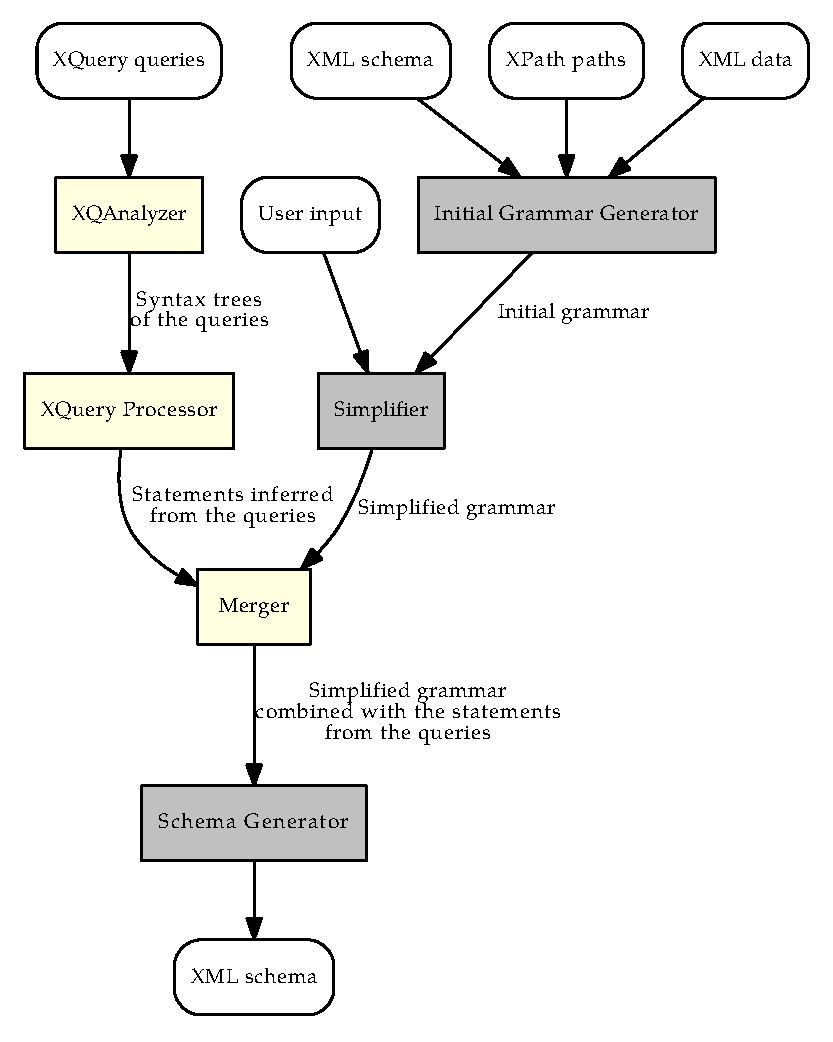
\includegraphics[scale=0.9]{jinfer_steps.eps}
\caption{jInfer process of inference}
\label{FIG_jinfer_steps}
\end{figure}

Figure \ref{FIG_jinfer_steps} shows the process of inference in jInfer. The grey and yellow rectangles represent steps of the inference, the white boxes represent input and output. Originally, the inference was composed of \textbf{Initial Grammar Generator}, \textbf{Simplifier}, and \textbf{Schema Generator} steps (grey). Steps (yellow) \textbf{XQAnalyzer}, \textbf{XQuery Processor}, and \textbf{Merger} are implementations of main parts of our proposed solution.

\begin{itemize}
\item \textbf{XQAnalyzer} - An implementation of the lexical and syntax analyses proposed in \cite{thesis_schejbal} and modified to create syntax trees. It parses input XQuery files and outputs their syntax trees.
\item \textbf{XQuery Processor} - An implementation of algorithms proposed in Chapter \ref{CHAPTER_proposed_algorithm}. In particular, construction of a syntax tree, static analysis of expression types, inference of built-in types, and key discovery. On input, it takes the syntax trees, and its output are statements inferred from the syntax tress. 
\item \textbf{Merger} - A step of inference responsible for combining the simplified grammar with the statements inferred by \textbf{XQuery Processor} as described in Chapter \ref{CHAPTER_combination_with_existings_methods_of_inference}, except the verification of types. Its result is the simplified grammar extended by the statements from \textbf{XQuery Processor} in a way that each statement is analysed and its information is assigned to concerned elements and attributes from the grammar. 
\end{itemize}

\section{jInfer Modules}
\begin{figure}
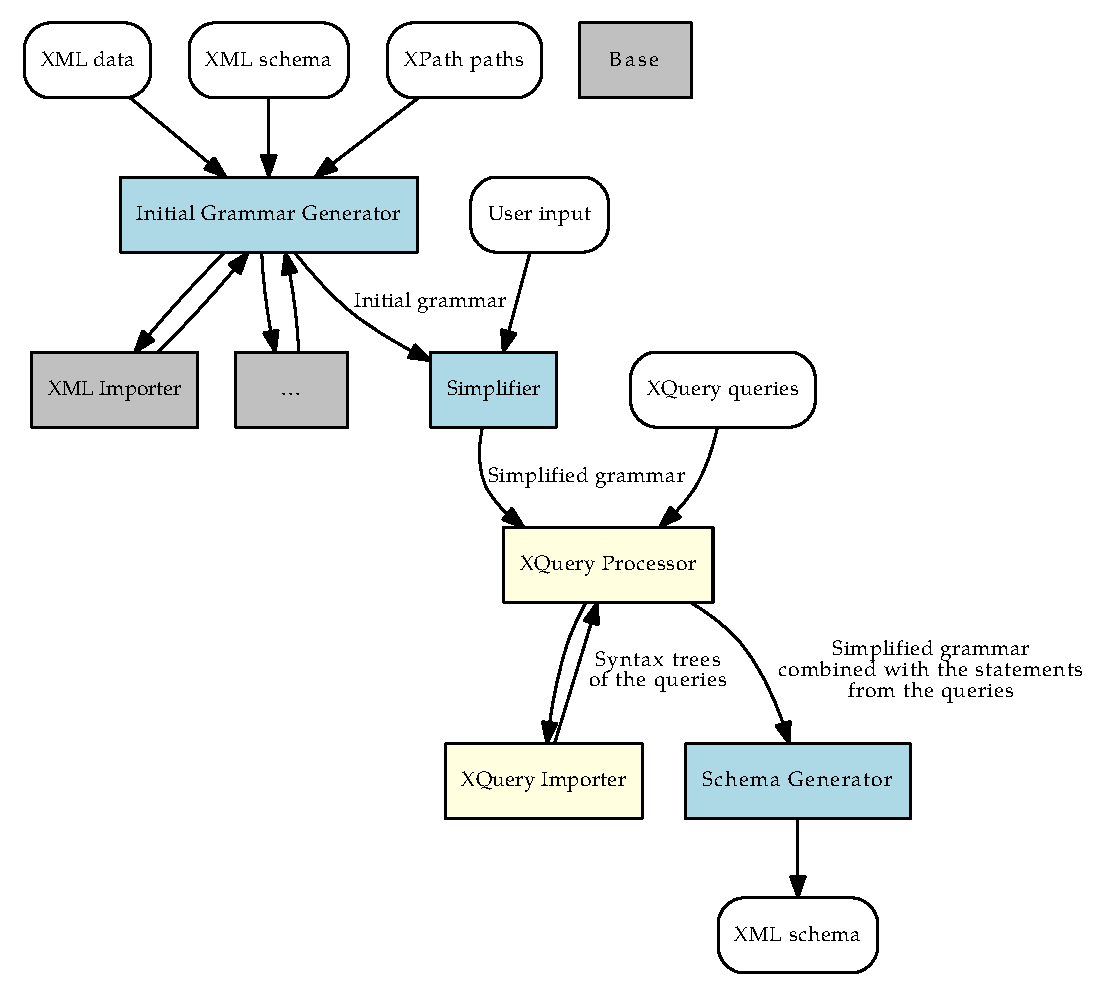
\includegraphics[scale=0.8]{jinfer_modules.eps}
\caption{jInfer modules}
\label{FIG_jinfer_modules}
\end{figure}

The previous section describes a high level schematic view of the process of inference. But, from a more technical view, jInfer modules do not utterly correspond with the steps of the presented process of inference.

The first difference is that none of the modules runs in parallel (in several threads) with other, as it is schematically shown in Figure \ref{FIG_jinfer_steps}. The modules run in a serial order as shown in Figure \ref{FIG_jinfer_modules}. The second difference is that one step is not always represented by one module, or one module is not always representing just one step.

Actually, the blue modules shown in Figure \ref{FIG_jinfer_modules} are module abstractions with specified interface. Actual modules are then implementations complying the interface. Since we provide only one implementation of modules for the proposed solution, this is not very important for this work and we do not describe the principle in detail. We only note that \textbf{Basic XQuery Processor} module is an implementation of \textbf{Non-grammatical Input Processor} module abstraction.

As in the previous section, newly added modules are those shown in yellow boxes. They are \textbf{Basic XQuery Processor} and \textbf{XQuery Importer}. We also modified modules \textbf{Basic XSD Exporter} (an implementation of \textbf{Schema Generator} interface) and \textbf{Base} to extend their functionality.

\begin{itemize}
\item \textbf{Base} - This is module containing common classes used by other modules and defining interfaces. We added five packages to this module. Package \texttt{cz.cuni.mff.ksi.jinfer.base.objects.xquery.syntaxtree.nodes} implements the structure of syntax trees. Package \texttt{cz.cuni.mff.ksi.jinfer\-.base.interfaces.xquery} contains \texttt{Type} interface which is an interface for types used in the type analysis of syntax trees. Package \texttt{cz.cuni.mff.ksi\-.jinfer.base\-.objects.xquery.types} contains implementations of \texttt{Type} interface and type utility classes. Package \texttt{cz.cuni.mff.ksi.jinfer\-.base\-.objects.xquery.keys} provides representations of keys and foreign keys, and package \texttt{cz.cuni.mff.ksi\-.jinfer.base.objects.xsd} provides representation of XSD built-in atomic types.
\item \textbf{XQuery Importer} - This module represents \textbf{XQAnalyzer} step in Figure \ref{FIG_jinfer_steps}. It is responsible for creating syntax trees from input XQuery files (step 1).
\item \textbf{Basic XQuery Processor} - The main module consisting of steps \textbf{XQuery Processor} and \textbf{Merger} in Figure \ref{FIG_jinfer_steps}. Package \texttt{cz.cuni.mff.ksi.jinfer\-.basicxqueryprocessor} contains the main module class \texttt{NonGrammatical\-InputProcessorImpl}. Other packages are \texttt{cz.cuni.mff.ksi.jinfer.\-basicxqueryprocessor.expressiontypesanalysis} implementing the static analysis of expression types (step 2), \texttt{cz.cuni.mff.ksi.jinfer.basic-\\xqueryprocessor.builtintype\-inference} implementing the inference of XSD built-in types (step 3), \texttt{cz\-.cuni.mff\-.ksi.jinfer\-.basicxquery-\\processor.keydiscovery} and their subpackages implementing the key discovery (step 4), \texttt{cz.cuni.mff.ksi.jinfer.basicxqueryprocessor.merger} implementing the merging with the grammar, and \texttt{cz.cuni.mff.ksi.jinfer\-.basicxqueryprocessor.utils} containing various utilities.
\item \textbf{Basic XSD Exporter} - This is the module responsible for generating the resulting schema in XSD. It was modified to process the additional information assigned to the grammar in \textbf{Basic XQuery Processor} module.
\end{itemize}
\chapter{Experiments} \label{CHAPTER_experiments}
In this chapter we describe how we performed experiments with the implementation and what problems we faced.

We made two test scenarios; one dealing with input data that were not made for purposes of this experiments, and the other extending the first dataset by data created for better test coverage.

\section{Test Scenario A}

\subsection{Test Data}
To get meaningful results of the experiments, test data should be composed of XML documents, which are instances of a certain, possibly not known, XML schema, and a set of XQuery queries which query the XML documents. The amount of the XML data does not have to be large. On the other hand, the set of queries should be large (at least hundreds of queries) and the queries should be real, not artificially made.

In a search for such test data, we have not succeeded. Large sets of XML data are available, but large sets of XQuery queries are not or it is not a simple task to obtain them.

If we cannot obtain an ideal set of test data, we can at least try to find the most suitable one from available non-ideal sets.

Sets of XML data and XQuery queries can be found in W3C XML Query Use Cases \cite{Marchiori:07:XQU}. However, those are very small sets of queries and the analysis of XQuery in Chapter \ref{CHAPTER_analysis_of_xquery} was worked out using those queries, and thus, the relevancy of such test data is questionable.

Another considered possibility was to obtain some set of XML data and create queries to it. This notion was rejected because such set would have all of the negative characteristics; it would be small, artificially made, and it would not be independent, as well.

At last, we concluded to use data provided by the XMark project \cite{xmark}. They are attached in Appendix \ref{APPENDIX_test_data} and they consists of automatically generated XML data and a set of twenty XQuery queries related to the data. Although, this set is also very small, it is more or less real and we did not known the set in the process of developing the algorithm.

\subsection{Results}

\subsubsection{Type Inference}
Six type statements shown in Table \ref{TAB_inferred_types} were inferred.

\begin{table}
\begin{tabular}{|l|}
\hline
\texttt{/site/open\_auctions/open\_auction/bidder/increase/text()} $\rightarrow$ \texttt{integer} \\ \hline
\texttt{/site/closed\_auctions/closed\_auction/price/text()} $\rightarrow$ \texttt{integer} \\ \hline
\texttt{/site/open\_auctions/open\_auction/initial/text()} $\rightarrow$ \texttt{integer} \\ \hline
\texttt{/site/open\_auctions/open\_auction/initial/text()} $\rightarrow$ \texttt{integer} \\ \hline
\texttt{/site/people/person/profile/@income} $\rightarrow$ \texttt{integer} \\ \hline
\texttt{/site/open\_auctions/open\_auction/reserve} $\rightarrow$ \texttt{decimal} \\ \hline
\end{tabular}
\caption{Inferred type statements A}
\label{TAB_inferred_types}
\end{table}

Only the last inferred statement is correct. Others are incorrect, because, comparing to the data, real type of nodes selected by the paths is \texttt{decimal}, as well.

To reveal the cause of the incorrect type inference, see, for example, query in Listing \ref{listing_test_query_12}. In the where clause, values of \texttt{/site/people/person/profile/\-@income} are compared to the integer literal constant \texttt{50000}. From this expression, it is not possible to infer the type correctly. The problem is that this is the only inferred statement. Better results can be achieved by providing a larger set of input queries, containing also expressions that can be exploited to infer correct statements. Then the verification with data can be incorporated to choose the correct statements.

\subsubsection{Key Discovery}
Four key statements and their normalized weights shown in Table \ref{TAB_inferred_keys} were inferred.

\begin{table}
\begin{tabular}{|l|c|}
\hline
\textbf{Key} & \textbf{Weight} \\ \hline \hline
\texttt{(/site/closed\_auctions/closed\_auction, \{buyer/@person\})} & -1.0 \\ \hline
\texttt{(/site/regions/europe/item, \{@id\})} & -0.417 \\ \hline
\texttt{(/site/people/person, \{@id\})} & 1.0 \\ \hline
\texttt{(/site/closed\_auctions/closed\_auction, \{itemref/@item\})} & 0.417 \\ \hline
\end{tabular}
\caption{Inferred key statements A}
\label{TAB_inferred_keys}
\end{table}

The first one is correct, a buyer is not a key of closed auctions. The second one is not correct, because \texttt{id} attribute is a key of \texttt{item} elements. The third one is correct and the fourth one declares \texttt{itemref} element to be a key of closed auctions, which is not true, but only with weight 0.417.

Closer analysis of input queries reveals that all of the statements were inferred from occurrences of the join pattern 3. That knowledge leads to the two following observations.

\begin{itemize}
\item The original method of key discovery would not infer anything on this input data.
\item The cause of the incorrectly inferred statements are not that they were inferred from join patterns occurrences, where a join is not done by a key/foreign key pair. It is that the for clauses (definitions of paths $P_1$ and $P_2$) in the join pattern 3 occurrence (in query in Listing \ref{listing_test_query_9}) are swapped, so the real key is considered as a foreign key and vice-versa.
\end{itemize}

A partial solution is an extension of the test data by queries containing expression that can be exploited to infer negative uniqueness statements. Such expression is, for example,\\ \texttt{distinct-values(/site/closed\_auctions/closed\_auction/itemref/@item)}\\ to get unique ids of items that was sold in some auction. Since, one item may be sold several times in auctions organized in different time periods, \texttt{distinct-values} function is applied.

From the original data, one negative uniqueness statement was inferred:\\
\texttt{/site/people/person/profile/interest/@category} is not unique with weight 1, and it it correct. Since, there is not such key statement inferred, the negative uniqueness statement is not used to any correction of weight.

\begin{table}
\begin{tabular}{|l|c|}
\hline
\textbf{Key} & \textbf{Weight} \\ \hline \hline
\texttt{(/site/closed\_auctions/closed\_auction, \{buyer/@person\})} & -1.0 \\ \hline
\texttt{(/site/regions/europe/item, \{@id\})} & -0.417 \\ \hline
\texttt{(/site/people/person, \{@id\})} & 1.0 \\ \hline
\texttt{(/site/closed\_auctions/closed\_auction, \{itemref/@item\})} & -0.417 \\ \hline
\end{tabular}
\caption{Key statements inferred from the extended test data A}
\label{TAB_inferred_keys_2}
\end{table}

From data extended by the mentioned expression, another negative uniqueness was inferred:\\
\texttt{/site/closed\_auctions/closed\_auction/itemref/@item} with weight 1. This one decreases the weight of the falsely inferred key. Key statements inferred from the extended data are shown in Table \ref{TAB_inferred_keys_2}.

As was demonstrated, larger sets of input data may lead to better results. However, the problem with the falsely rejected key still remains. It may be solved by modification of the statements inferred from occurrences of the join pattern 3. If we omit the negative statement of a key from the second for clause ($(P_2, \{L_2\})$ is not satisfied), we get better results. The modified statements inferred from an occurrence of the join pattern 3 are the following (assigned weight remains 0.5):

\begin{itemize}
\item $(P_1, \{L_1\})$ is satisfied
\item $(P_2, \{L_2\}) \rightarrow (P_1, \{L_1\})$ is satisfied
\end{itemize}

From the extended test data, using the modified join pattern 3 statements, key statements in Table \ref{TAB_inferred_keys_3} were inferred. Those are the best results from all test runs, though it is not clear that the modified statements will produce the best results also on other larger input data. Therefore, further tests with large sets of queries are required to determine the best settings for the algorithm. 

\begin{table}
\begin{tabular}{|l|c|}
\hline
\textbf{Key} & \textbf{Weight} \\ \hline \hline
\texttt{(/site/people/person, \{@id\})} & 1.0 \\ \hline
\texttt{(/site/closed\_auctions/closed\_auction, \{itemref/@item\})} & -0.333 \\ \hline
\end{tabular}
\caption[Key statements inferred using the modified JP3 statements]{Key statements inferred from the extended test data using the modified JP3 statements}
\label{TAB_inferred_keys_3}
\end{table}

\section{Test Scenario B}
As mentioned before, the previous test scenario involves only data with JP3 occurrences, and therefore, it only tests the extension of the original method, while the original method itself remains untested. To correct it, we add several new test queries created by ourselves.

\subsection{Test Data}

\begin{lstlisting}[caption=Test query B1 containing a for join pattern occurrence., frame=single, label=listing_test_query_b1]
for $item in /site/regions/europe/item
let $closed_auctions := /site/closed_auctions/closed_auction[itemref/@item = $item/@id]
return <item><id>{$item/@id}</id><max-price>{max($closed_auctions/price)}</max-price></item>
\end{lstlisting}

\begin{lstlisting}[caption=Test query B2 containing a let join pattern occurrence., frame=single, label=listing_test_query_b2]
for $open_auction in /site/open_auctions/open_auction
let $item := /site/regions/europe/item[@id = $open_auction/itemref/@item]
return $item/personref/@person
\end{lstlisting}

\begin{lstlisting}[caption=Test query B3 containing let join pattern and JP3 occurrences., frame=single, label=listing_test_query_b3, numbers=left, numberstyle=\tiny]
for $person in /site/people/person
where $person/profile/@income < 100.00 and $person/profile/gender = "m"
return
    <list>{
        for $auction in /site/closed_auctions/closed_auction
        let $item := /site//item[@id = $auction/itemref/@item]
        let $price := $auction/price
        where $auction/buyer/@person = $person/@id
        return
            <record><person>{$person/@id}</person><item>{$item/@id}</item><price>{$price}</price></record>
    }</list>
\end{lstlisting}

In this scenario, we use test data from the Test Scenario A extended by queries in Listings \ref{listing_test_query_b1}, \ref{listing_test_query_b2}, and \ref{listing_test_query_b3}.

The first two ones are simple queries containing one join pattern occurrence each. The third one contains occurrences of let join pattern (binding clauses at lines 5 and 6) and JP3 (binding clauses at lines 1 and 5, and where clause at line 8), two expressions exploitable by the inference of types (both at line 2) and one negative uniqueness statement of the comparison-with-a-constant form (comparison with \texttt{"m"} at line 2). Thus, the third query contains instances of all types of the constructs utilized by our method.

\subsubsection{Results}

\begin{table}
\begin{tabular}{|l|}
\hline
\texttt{/site/open\_auctions/open\_auction/bidder/increase/text()} $\rightarrow$ \texttt{integer} \\ \hline
\texttt{/site/closed\_auctions/closed\_auction/price/text()} $\rightarrow$ \texttt{integer} \\ \hline
\texttt{/site/open\_auctions/open\_auction/initial/text()} $\rightarrow$ \texttt{integer} \\ \hline
\texttt{/site/open\_auctions/open\_auction/initial/text()} $\rightarrow$ \texttt{integer} \\ \hline
\texttt{/site/people/person/profile/@income} $\rightarrow$ \texttt{integer} \\ \hline
\texttt{/site/open\_auctions/open\_auction/reserve} $\rightarrow$ \texttt{decimal} \\ \hline
\texttt{/site/people/person/profile/@income} $\rightarrow$ \texttt{decimal} \\ \hline
\texttt{/site/people/person/profile/gender} $\rightarrow$ \texttt{string} \\ \hline
\end{tabular}
\caption{Inferred type statements B}
\label{TAB_inferred_types_b}
\end{table}

\begin{table}
\begin{tabular}{|l|c|}
\hline
\textbf{Key} & \textbf{Weight} \\ \hline \hline
\texttt{(/site//item, {@id})} & 0.333 \\ \hline
\texttt{(/site/people/person, {@id})} & 0.6 \\ \hline
\texttt{(/site/closed\_auctions/closed\_auction, {buyer/@person})} & -0.6 \\ \hline
\texttt{(/site/closed\_auctions/closed\_auction, {itemref/@item})} & -0.917 \\ \hline
\texttt{(/site/regions/europe/item, {@id})} & 0.6 \\ \hline
\end{tabular}
\caption{Inferred key statements B}
\label{TAB_inferred_keys_b}
\end{table}

\begin{table}
\begin{tabular}{|l|c|}
\hline
\textbf{Node} & \textbf{Weight} \\ \hline \hline
\texttt{(/site/people/person/profile/interest/@category)} & 1 \\ \hline
\texttt{(/site/closed\_auctions/closed\_auction/itemref/@item)} & 1 \\ \hline
\texttt{(/site/people/person/profile/gender)} & 0.9 \\ \hline
\end{tabular}
\caption{Inferred negative uniqueness statements B}
\label{TAB_inferred_negative_uniqueness_statements_b}
\end{table}

Results of this test scenario are shown in Tables \ref{TAB_inferred_types_b}, \ref{TAB_inferred_keys_b}, and \ref{TAB_inferred_negative_uniqueness_statements_b}. All seem to be as we expected.

Note that all inferred type statements are correct, however, the weight of the \texttt{(/site//item, {@id})} key is only 0.333. The reason is that there is only one join pattern occurrence resulting to this key, and therefore in summary, its normalized weight is low and it is correct.

We demonstrated that also the original method works and we can get better results with little larger input dataset. Though, this set is still very small and we do not show how the methods work with large real-world data, possibly containing FLWOR constructs not satisfying our assumption that each join is done by a key/foreign key pair.

We attach the resulting XSD in Appendix \ref{listing_xsd}. It was made using threshold 0.3. It means that all key statements with normalized weight equal or higher than 0.3 are considered correct and are included in the schema.
\chapter{Conclusion}
The aim of this thesis was to employ XML operations in the XML schema inference. We analyzed several existing methods of the XML schema inference and we searched for methods that utilize some XML operations. We found only one method, inferring keys from XQuery queries.

Since the notion of XML operations is very general and the range of XML technologies is very large, for the purpose of this work, we decided to focus on XQuery technology. We made the overview of possible utilization of XQuery queries in the process of XML schema inference.

Before a creation of the algorithm itself, we had to take several decisions in questions that emerged. Since there is a lack of the methods dealing with the utilisation of XML operation, there is also a lack of practically proven solutions that can help in such decision making.

In the proposed solution, we decided to incorporate lexical and syntax analyses of XQuery queries, because it is more general and more extensible than a pattern searching. To achieve that, we adopted the algorithm from a recent master thesis dealing with an analysis of XQuery queries.

We also implemented several ideas from the overview to infer XSD built-in types of elements and attributes. And we extended and implemented the one existing method dealing with the inference of keys. We experimentally demonstrated that on some input files, results of the extended method are better than results of the original method. However, we did not succeed in a search of an ideal, large enough set of test data. The testing was performed on a small set of input queries and further testing and algorithm tuning is required.

Finally, we proposed a simple way how to combine the inferred statements with existing grammar inferring methods of the XML schema inference and we implemented it using the jInfer framework. Thus, we created the first complete, ready-to-use, and extensible implementation of the XML xchema inference exploiting XQuery queries besides XML data.

\todo[inline]{Nejake prehladne zhrnutie plusov a minusov?}

\section{Future Work}
This work implements only some ideas discussed in the overview in Chapter \ref{CHAPTER_analysis_of_xquery}, leaving most of them for a future work. Also, the implemented algorithms can be further refined as was already mentioned in Chapter \ref{CHAPTER_proposed_algorithm} with the presentation of the algorithms. For example thorough processing of user-defined function calls.

Chapter \ref{CHAPTER_precreation_of_algorithm} discusses some possible future enhancements as well. A research on possibilities of modifying the grammar rules based on information extracted from XQuery queries may bring interesting results. We analyse the queries statically only, we do not evaluate them. An analysis of queries together with their results can be a topic of another future research direction.

The utilization of XQuery queries certainly provides a space for incorporating an interaction with user. For example, a user may influence the scoring of inferred keys to get more precise results.

And, a very large space for a possible future research is provided by utilisation of other XML operations. The main representant is XSLT.

Besides the mentioned, our opinion is that the most urgent future work is obtaining a large enough test data set, performing proper experiments, and refining the algorithm by modification of its settings (statements inferred from join pattern occurrences, weights, etc.) according to experimental results. This process was suggested in Chapter \ref{CHAPTER_experiments}.

%%% Seznam pouľité literatury
\nocite{*}
\bibliographystyle{plain}
\bibliography{literature}

%%% Pouľité zkratky v diplomové práci, existují-li, včetně jejich vysvětlení.
%\chapwithtoc{List of Abbreviations}
%\todo[inline]{Není nutno.}

%%% Přílohy k diplomové práci, existují-li (různé dodatky jako výpisy programů,
%%% diagramy apod.). Kaľdá příloha musí být alespoň jednou odkazována z vlastního
%%% textu práce. Přílohy se číslují.
%\chapwithtoc{Attachments}
\appendix
\chapter{Attachments}
\begin{figure}[float=htpb]
Logical: \texttt{AND}, \texttt{OR}.

Comparison: \texttt{GEN\_EQUALS}, \texttt{GEN\_NOT\_EQUALS}, \texttt{GEN\_LESS\_THAN}, \texttt{GEN\_LESS\_THAN\_EQUALS}, \texttt{GEN\_GREATER\_THAN}, \texttt{GEN\_GREATER\_THAN\_EQUALS}, \texttt{VAL\_EQUALS}, \texttt{VAL\_NOT\_EQUALS}, \texttt{VAL\_LESS\_THAN}, \texttt{VAL\_LESS\_THAN\_EQUALS}, \texttt{VAL\_GREATER\_THAN}, \texttt{VAL\_GREATER\_THAN\_EQUALS}, \texttt{NOD\_IS}, \texttt{NOD\_PRECEDES}, \texttt{NOD\_FOLLOWS}.

Range: \texttt{TO}.

Additive: \texttt{PLUS}, \texttt{MINUS}.

Multiplicative: \texttt{MUL}, \texttt{DIV}, \texttt{IDIV}, \texttt{MOD}.

Set: \texttt{UNION}, \texttt{INTERSECTION}, \texttt{DIFFERENCE}.

Type test: \texttt{INSTANCE\_OF}, \texttt{CASTABLE\_AS}.

Type conversion: \texttt{TREAT\_AS}, \texttt{CAST\_AS}.

Unary: \texttt{UNARY\_PLUS}, \texttt{UNARY\_MINUS}.
\caption[String representations of operators in syntax tree]{All possible values representing an operator in an instance of \texttt{OperatorNode}}
\label{FIG_operators}
\end{figure}


\begin{lstlisting}[caption=Resulting XSD of Test Scenario B, frame=single, label=listing_xsd]
<?xml version="1.0" encoding="UTF-8"?>
<xs:schema xmlns:xs="http://www.w3.org/2001/XMLSchema">
<!-- Inferred on Sat Mar 31 21:28:32 CEST 2012 by Basic IG generator, TwoStep(Iname (with attributes), Automaton Merging State(GreedyMDL(Combined(k,h-context, s,k-strings, Null, Null),Naive Alphabet), State Removal Ordered(Weighted)), Chained(Empty Children, Nested Concatenation, Null)), Basic XSD exporter -->

<!-- global types -->
<xs:complexType name="Temph" mixed="true">
  <xs:sequence>
    <xs:sequence minOccurs="0" maxOccurs="unbounded">
      <xs:choice>
        <xs:element name="keyword" type="Tkeyword"/>
        <xs:element name="bold" type="Tbold"/>
      </xs:choice>
    </xs:sequence>
  </xs:sequence>
</xs:complexType>

<xs:complexType name="Tbold" mixed="true">
  <xs:sequence>
    <xs:choice>
      <xs:choice>
        <xs:sequence>
          <xs:element name="emph" type="Temph"/>
        </xs:sequence>
      </xs:choice>
      <xs:sequence>
        <xs:element name="keyword" type="Tkeyword"/>
      </xs:sequence>
    </xs:choice>
  </xs:sequence>
</xs:complexType>

<xs:complexType name="Tkeyword" mixed="true">
  <xs:sequence>
    <xs:choice>
      <xs:sequence minOccurs="0">
        <xs:element name="bold" type="Tbold"/>
      </xs:sequence>
      <xs:sequence>
        <xs:element name="emph" type="Temph"/>
      </xs:sequence>
    </xs:choice>
  </xs:sequence>
</xs:complexType>

<xs:complexType name="Ttext" mixed="true">
  <xs:choice minOccurs="0" maxOccurs="unbounded">
    <xs:element name="bold" type="Tbold"/>
    <xs:element name="keyword" type="Tkeyword"/>
    <xs:element name="emph" type="Temph"/>
  </xs:choice>
</xs:complexType>

<xs:complexType name="Tparlist">
  <xs:sequence>
    <xs:element name="listitem" type="Tlistitem" minOccurs="0" maxOccurs="unbounded"/>
  </xs:sequence>
</xs:complexType>

<xs:complexType name="Tlistitem">
  <xs:choice>
    <xs:element name="text" type="Ttext"/>
    <xs:element name="parlist" type="Tparlist"/>
  </xs:choice>
</xs:complexType>

<xs:complexType name="Tdescription">
  <xs:choice>
    <xs:element name="parlist" type="Tparlist"/>
    <xs:element name="text" type="Ttext"/>
  </xs:choice>
</xs:complexType>

<xs:complexType name="Tincategory">
  <xs:attribute name="category" type="xs:string" use="required"/>
</xs:complexType>

<xs:complexType name="Tmail">
  <xs:sequence>
    <xs:element name="from" type="xs:string"/>
    <xs:element name="to" type="xs:string"/>
    <xs:element name="date" type="xs:string"/>
    <xs:element name="text" type="Ttext"/>
  </xs:sequence>
</xs:complexType>

<xs:complexType name="Tmailbox">
  <xs:sequence minOccurs="0">
    <xs:element name="mail" type="Tmail"/>
    <xs:element name="mail" type="Tmail" minOccurs="0"/>
  </xs:sequence>
</xs:complexType>

<xs:complexType name="Titem">
  <xs:sequence>
    <xs:element name="location" type="xs:string"/>
    <xs:element name="quantity" type="xs:string"/>
    <xs:element name="name" type="xs:string"/>
    <xs:element name="payment" type="xs:string"/>
    <xs:element name="description" type="Tdescription"/>
    <xs:element name="shipping" type="xs:string"/>
    <xs:element name="incategory" type="Tincategory" minOccurs="0" maxOccurs="unbounded"/>
    <xs:element name="mailbox" type="Tmailbox"/>
  </xs:sequence>
  <xs:attribute name="id" type="xs:string" use="required"/>
</xs:complexType>

<xs:complexType name="Tafrica">
  <xs:sequence>
    <xs:element name="item" type="Titem"/>
  </xs:sequence>
</xs:complexType>

<xs:complexType name="Tasia">
  <xs:sequence>
    <xs:element name="item" type="Titem"/>
    <xs:element name="item" type="Titem"/>
  </xs:sequence>
</xs:complexType>

<xs:complexType name="Taustralia">
  <xs:sequence>
    <xs:element name="item" type="Titem"/>
    <xs:element name="item" type="Titem"/>
  </xs:sequence>
</xs:complexType>

<xs:complexType name="Teurope">
  <xs:sequence>
    <xs:element name="item" type="Titem" minOccurs="0" maxOccurs="unbounded"/>
  </xs:sequence>
</xs:complexType>

<xs:complexType name="Tnamerica">
  <xs:sequence>
    <xs:element name="item" type="Titem" minOccurs="0" maxOccurs="unbounded"/>
  </xs:sequence>
</xs:complexType>

<xs:complexType name="Tsamerica">
  <xs:sequence>
    <xs:element name="item" type="Titem"/>
  </xs:sequence>
</xs:complexType>

<xs:complexType name="Tregions">
  <xs:sequence>
    <xs:element name="africa" type="Tafrica"/>
    <xs:element name="asia" type="Tasia"/>
    <xs:element name="australia" type="Taustralia"/>
    <xs:element name="europe" type="Teurope"/>
    <xs:element name="namerica" type="Tnamerica"/>
    <xs:element name="samerica" type="Tsamerica"/>
  </xs:sequence>
</xs:complexType>

<xs:complexType name="Tcategory">
  <xs:sequence>
    <xs:element name="name" type="xs:string"/>
    <xs:element name="description" type="Tdescription"/>
  </xs:sequence>
  <xs:attribute name="id" type="xs:string" use="required"/>
</xs:complexType>

<xs:complexType name="Tcategories">
  <xs:sequence>
    <xs:element name="category" type="Tcategory"/>
  </xs:sequence>
</xs:complexType>

<xs:complexType name="Tedge">
  <xs:attribute name="from" type="xs:string" use="required"/>
  <xs:attribute name="to" type="xs:string" use="required"/>
</xs:complexType>

<xs:complexType name="Tcatgraph">
  <xs:sequence>
    <xs:element name="edge" type="Tedge"/>
  </xs:sequence>
</xs:complexType>

<xs:complexType name="Taddress">
  <xs:sequence>
    <xs:element name="street" type="xs:string"/>
    <xs:element name="city" type="xs:string"/>
    <xs:element name="country" type="xs:string"/>
    <xs:choice>
      <xs:element name="zipcode" type="xs:string"/>
      <xs:sequence>
        <xs:element name="province" type="xs:string"/>
        <xs:element name="zipcode" type="xs:string"/>
      </xs:sequence>
    </xs:choice>
  </xs:sequence>
</xs:complexType>

<xs:complexType name="Tinterest">
  <xs:attribute name="category" type="xs:string" use="required"/>
</xs:complexType>

<xs:complexType name="Tprofile">
  <xs:sequence>
    <xs:choice minOccurs="0" maxOccurs="unbounded">
      <xs:element name="education" type="xs:string"/>
      <xs:element name="interest" type="Tinterest"/>
    </xs:choice>
    <xs:choice>
      <xs:element name="business" type="xs:string"/>
      <xs:sequence>
        <xs:element name="gender" type="xs:string"/>
        <xs:element name="business" type="xs:string"/>
      </xs:sequence>
    </xs:choice>
    <xs:element name="age" type="xs:string" minOccurs="0"/>
  </xs:sequence>
  <xs:attribute name="income" type="xs:integer" use="required"/>
</xs:complexType>

<xs:complexType name="Twatch">
  <xs:attribute name="open_auction" type="xs:string" use="required"/>
</xs:complexType>

<xs:complexType name="Twatches">
  <xs:sequence>
    <xs:element name="watch" type="Twatch" minOccurs="0" maxOccurs="unbounded"/>
  </xs:sequence>
</xs:complexType>

<xs:complexType name="Tperson">
  <xs:sequence>
    <xs:element name="name" type="xs:string"/>
    <xs:element name="emailaddress" type="xs:string"/>
    <xs:choice minOccurs="0" maxOccurs="unbounded">
      <xs:element name="address" type="Taddress"/>
      <xs:element name="phone" type="xs:string"/>
      <xs:element name="homepage" type="xs:string"/>
      <xs:element name="creditcard" type="xs:string"/>
    </xs:choice>
    <xs:choice>
      <xs:sequence minOccurs="0">
        <xs:element name="profile" type="Tprofile"/>
        <xs:element name="watches" type="Twatches" minOccurs="0"/>
      </xs:sequence>
      <xs:element name="watches" type="Twatches"/>
    </xs:choice>
  </xs:sequence>
  <xs:attribute name="id" type="xs:string" use="required"/>
</xs:complexType>

<xs:complexType name="Tpeople">
  <xs:sequence>
    <xs:element name="person" type="Tperson" minOccurs="0" maxOccurs="unbounded"/>
  </xs:sequence>
</xs:complexType>

<xs:complexType name="Tpersonref">
  <xs:attribute name="person" type="xs:string" use="required"/>
</xs:complexType>

<xs:complexType name="Tbidder">
  <xs:sequence>
    <xs:element name="date" type="xs:string"/>
    <xs:element name="time" type="xs:string"/>
    <xs:element name="personref" type="Tpersonref"/>
    <xs:element name="increase" type="xs:integer"/>
  </xs:sequence>
</xs:complexType>

<xs:complexType name="Titemref">
  <xs:attribute name="item" type="xs:string" use="required"/>
</xs:complexType>

<xs:complexType name="Tseller">
  <xs:attribute name="person" type="xs:string" use="required"/>
</xs:complexType>

<xs:complexType name="Tauthor">
  <xs:attribute name="person" type="xs:string" use="required"/>
</xs:complexType>

<xs:complexType name="Tannotation">
  <xs:sequence>
    <xs:element name="author" type="Tauthor"/>
    <xs:element name="description" type="Tdescription"/>
    <xs:element name="happiness" type="xs:string"/>
  </xs:sequence>
</xs:complexType>

<xs:complexType name="Tinterval">
  <xs:sequence>
    <xs:element name="start" type="xs:string"/>
    <xs:element name="end" type="xs:string"/>
  </xs:sequence>
</xs:complexType>

<xs:complexType name="Topen_auction">
  <xs:sequence>
    <xs:element name="initial" type="xs:integer"/>
    <xs:choice minOccurs="0" maxOccurs="unbounded">
      <xs:element name="reserve" type="xs:decimal"/>
      <xs:element name="bidder" type="Tbidder"/>
    </xs:choice>
    <xs:element name="current" type="xs:string"/>
    <xs:element name="privacy" type="xs:string" minOccurs="0" maxOccurs="unbounded"/>
    <xs:element name="itemref" type="Titemref"/>
    <xs:element name="seller" type="Tseller"/>
    <xs:element name="annotation" type="Tannotation"/>
    <xs:element name="quantity" type="xs:string"/>
    <xs:element name="type" type="xs:string"/>
    <xs:element name="interval" type="Tinterval"/>
  </xs:sequence>
  <xs:attribute name="id" type="xs:string" use="required"/>
</xs:complexType>

<xs:complexType name="Topen_auctions">
  <xs:sequence>
    <xs:element name="open_auction" type="Topen_auction" minOccurs="0" maxOccurs="unbounded"/>
  </xs:sequence>
</xs:complexType>

<xs:complexType name="Tbuyer">
  <xs:attribute name="person" type="xs:string" use="required"/>
</xs:complexType>

<xs:complexType name="Tclosed_auction">
  <xs:sequence>
    <xs:element name="seller" type="Tseller"/>
    <xs:element name="buyer" type="Tbuyer"/>
    <xs:element name="itemref" type="Titemref"/>
    <xs:element name="price" type="xs:integer"/>
    <xs:element name="date" type="xs:string"/>
    <xs:element name="quantity" type="xs:string"/>
    <xs:element name="type" type="xs:string"/>
    <xs:element name="annotation" type="Tannotation"/>
  </xs:sequence>
</xs:complexType>

<xs:complexType name="Tclosed_auctions">
  <xs:sequence>
    <xs:element name="closed_auction" type="Tclosed_auction" minOccurs="0" maxOccurs="unbounded"/>
  </xs:sequence>
</xs:complexType>

<xs:complexType name="Tsite">
  <xs:sequence>
    <xs:element name="regions" type="Tregions"/>
    <xs:element name="categories" type="Tcategories"/>
    <xs:element name="catgraph" type="Tcatgraph"/>
    <xs:element name="people" type="Tpeople"/>
    <xs:element name="open_auctions" type="Topen_auctions"/>
    <xs:element name="closed_auctions" type="Tclosed_auctions"/>
  </xs:sequence>
</xs:complexType>

<!-- top level element -->
<xs:element name="site" type="Tsite">
  <xs:key name="key1">
    <xs:selector xpath="people/person"/>
    <xs:field xpath="@id"/>
  </xs:key>
  <xs:key name="key2">
    <xs:selector xpath=".//item"/>
    <xs:field xpath="@id"/>
  </xs:key>
  <xs:key name="key3">
    <xs:selector xpath="regions/europe/item"/>
    <xs:field xpath="@id"/>
  </xs:key>
  <xs:keyref name="keyRef1_key1" refer="key1">
    <xs:selector xpath="closed_auctions/closed_auction"/>
    <xs:field xpath="buyer/@person"/>
  </xs:keyref>
  <xs:keyref name="keyRef2_key2" refer="key2">
    <xs:selector xpath="closed_auctions/closed_auction"/>
    <xs:field xpath="itemref/@item"/>
  </xs:keyref>
  <xs:keyref name="keyRef3_key3" refer="key3">
    <xs:selector xpath="closed_auctions/closed_auction"/>
    <xs:field xpath="itemref/@item"/>
  </xs:keyref>
  <xs:keyref name="keyRef4_key3" refer="key3">
    <xs:selector xpath="open_auctions/open_auction"/>
    <xs:field xpath="itemref/@item"/>
  </xs:keyref>
</xs:element>
</xs:schema>
\end{lstlisting}
\chapter{Test Data} \label{APPENDIX_test_data}

Test data from the XMark project \cite{xmark}. Using the provided XML generator, XML document of size approximately 1.5 MB was generated. Figure \ref{listing_dtd} is its DTD and other figures in this appendix are XQuery queries that query the XML document.

The queries was slightly modified by replacing calls of \texttt{doc} function in paths by \texttt{/} (document node).

\begin{lstlisting}[caption=DTD of the test XML data, frame=single, label=listing_dtd]
<!-- DTD for auction database -->
<!-- $Id: auction.dtd,v 1.15 2001/01/29 21:42:35 albrecht Exp $ -->

<!ELEMENT site            (regions, categories, catgraph, people, open_auctions, closed_auctions)>

<!ELEMENT categories      (category+)>
<!ELEMENT category        (name, description)>
<!ATTLIST category        id ID #REQUIRED>
<!ELEMENT name            (#PCDATA)>
<!ELEMENT description     (text | parlist)>
<!ELEMENT text            (#PCDATA | bold | keyword | emph)*>
<!ELEMENT bold            (#PCDATA | bold | keyword | emph)*>
<!ELEMENT keyword         (#PCDATA | bold | keyword | emph)*>
<!ELEMENT emph            (#PCDATA | bold | keyword | emph)*>
<!ELEMENT parlist         (listitem)*>
<!ELEMENT listitem        (text | parlist)*>

<!ELEMENT catgraph        (edge*)>
<!ELEMENT edge            EMPTY>
<!ATTLIST edge            from IDREF #REQUIRED to IDREF #REQUIRED>

<!ELEMENT regions         (africa, asia, australia, europe, namerica, samerica)>
<!ELEMENT africa          (item*)>
<!ELEMENT asia            (item*)>
<!ELEMENT australia       (item*)>
<!ELEMENT namerica        (item*)>
<!ELEMENT samerica        (item*)>
<!ELEMENT europe          (item*)>
<!ELEMENT item            (location, quantity, name, payment, description, shipping, incategory+, mailbox)>
<!ATTLIST item            id ID #REQUIRED
                          featured CDATA #IMPLIED>
<!ELEMENT location        (#PCDATA)>
<!ELEMENT quantity        (#PCDATA)>
<!ELEMENT payment         (#PCDATA)>
<!ELEMENT shipping        (#PCDATA)>
<!ELEMENT reserve         (#PCDATA)>
<!ELEMENT incategory      EMPTY>
<!ATTLIST incategory      category IDREF #REQUIRED>
<!ELEMENT mailbox         (mail*)>
<!ELEMENT mail            (from, to, date, text)>
<!ELEMENT from            (#PCDATA)>
<!ELEMENT to              (#PCDATA)>
<!ELEMENT date            (#PCDATA)>
<!ELEMENT itemref         EMPTY>
<!ATTLIST itemref         item IDREF #REQUIRED>
<!ELEMENT personref       EMPTY>
<!ATTLIST personref       person IDREF #REQUIRED>

<!ELEMENT people          (person*)>
<!ELEMENT person          (name, emailaddress, phone?, address?, homepage?, creditcard?, profile?, watches?)>
<!ATTLIST person          id ID #REQUIRED>
<!ELEMENT emailaddress    (#PCDATA)>
<!ELEMENT phone           (#PCDATA)>
<!ELEMENT address         (street, city, country, province?, zipcode)>
<!ELEMENT street          (#PCDATA)>
<!ELEMENT city            (#PCDATA)>
<!ELEMENT province        (#PCDATA)>
<!ELEMENT zipcode         (#PCDATA)>
<!ELEMENT country         (#PCDATA)>
<!ELEMENT homepage        (#PCDATA)>
<!ELEMENT creditcard      (#PCDATA)>
<!ELEMENT profile         (interest*, education?, gender?, business, age?)>
<!ATTLIST profile         income CDATA #IMPLIED>
<!ELEMENT interest        EMPTY>
<!ATTLIST interest        category IDREF #REQUIRED>
<!ELEMENT education       (#PCDATA)>
<!ELEMENT income          (#PCDATA)>
<!ELEMENT gender          (#PCDATA)>
<!ELEMENT business        (#PCDATA)>
<!ELEMENT age             (#PCDATA)>
<!ELEMENT watches         (watch*)>
<!ELEMENT watch           EMPTY>
<!ATTLIST watch           open_auction IDREF #REQUIRED>

<!ELEMENT open_auctions   (open_auction*)>
<!ELEMENT open_auction    (initial, reserve?, bidder*, current, privacy?, itemref, seller, annotation, quantity, type, interval)>
<!ATTLIST open_auction    id ID #REQUIRED>
<!ELEMENT privacy         (#PCDATA)>
<!ELEMENT initial         (#PCDATA)>
<!ELEMENT bidder          (date, time, personref, increase)>
<!ELEMENT seller          EMPTY>
<!ATTLIST seller          person IDREF #REQUIRED>
<!ELEMENT current         (#PCDATA)>
<!ELEMENT increase        (#PCDATA)>
<!ELEMENT type            (#PCDATA)>
<!ELEMENT interval        (start, end)>
<!ELEMENT start           (#PCDATA)>
<!ELEMENT end             (#PCDATA)>
<!ELEMENT time            (#PCDATA)>
<!ELEMENT status          (#PCDATA)>
<!ELEMENT amount          (#PCDATA)>

<!ELEMENT closed_auctions (closed_auction*)>
<!ELEMENT closed_auction  (seller, buyer, itemref, price, date, quantity, type, annotation?)>
<!ELEMENT buyer           EMPTY>
<!ATTLIST buyer           person IDREF #REQUIRED>
<!ELEMENT price           (#PCDATA)>
<!ELEMENT annotation      (author, description?, happiness)>

<!ELEMENT author          EMPTY>
<!ATTLIST author          person IDREF #REQUIRED>
<!ELEMENT happiness       (#PCDATA)>
\end{lstlisting}

\begin{lstlisting}[caption=Test query 1., frame=single, label=listing_test_query_1]
for $b in /site/people/person[@id = "person0"] return $b/name/text()
\end{lstlisting}

\begin{lstlisting}[caption=Test query 2., frame=single, label=listing_test_query_2]
for $b in /site/open_auctions/open_auction
return <increase>{$b/bidder[1]/increase/text()}</increase>
\end{lstlisting}

\begin{lstlisting}[caption=Test query 3., frame=single, label=listing_test_query_3]
for $b in /site/open_auctions/open_auction
where zero-or-one($b/bidder[1]/increase/text()) * 2 <= $b/bidder[last()]/increase/text()
return
  <increase
  first="{$b/bidder[1]/increase/text()}"
  last="{$b/bidder[last()]/increase/text()}"/>
\end{lstlisting}

\begin{lstlisting}[float=htpb, caption=Test query 4., frame=single, label=listing_test_query_4]
for $b in /site/open_auctions/open_auction
where
  some $pr1 in $b/bidder/personref[@person = "person20"],
       $pr2 in $b/bidder/personref[@person = "person51"]
  satisfies $pr1 << $pr2
return <history>{$b/reserve/text()}</history>
\end{lstlisting}

\begin{lstlisting}[float=htpb, caption=Test query 5., frame=single, label=listing_test_query_5]
count(
  for $i in /site/closed_auctions/closed_auction
  where $i/price/text() >= 40
  return $i/price
)
\end{lstlisting}

\begin{lstlisting}[float=htpb, caption=Test query 6., frame=single, label=listing_test_query_6]
for $b in //site/regions return count($b//item)
\end{lstlisting}

\begin{lstlisting}[float=htpb, caption=Test query 7., frame=single, label=listing_test_query_7]
for $p in /site
return
  count($p//description) + count($p//annotation) + count($p//emailaddress)
\end{lstlisting}

\begin{lstlisting}[float=htpb, caption=Test query 8., frame=single, label=listing_test_query_8]
for $p in /site/people/person
let $a :=
  for $t in /site/closed_auctions/closed_auction
  where $t/buyer/@person = $p/@id
  return $t
return <item person="{$p/name/text()}">{count($a)}</item>
\end{lstlisting}

\begin{lstlisting}[float=htpb, caption=Test query 9., frame=single, label=listing_test_query_9]
let $ca := /site/closed_auctions/closed_auction return
let
    $ei := /site/regions/europe/item
for $p in /site/people/person
let $a :=
  for $t in $ca
  where $p/@id = $t/buyer/@person
  return
    let $n := for $t2 in $ei where $t/itemref/@item = $t2/@id return $t2
    return <item>{$n/name/text()}</item>
return <person name="{$p/name/text()}">{$a}</person>
\end{lstlisting}

\begin{lstlisting}[float=htpb, caption=Test query 10., frame=single, label=listing_test_query_10]
for $i in
  distinct-values(/site/people/person/profile/interest/@category)
let $p :=
  for $t in /site/people/person
  where $t/profile/interest/@category = $i
  return
    <personne>
      <statistiques>
        <sexe>{$t/profile/gender/text()}</sexe>
        <age>{$t/profile/age/text()}</age>
        <education>{$t/profile/education/text()}</education>
        <revenu>{fn:data($t/profile/@income)}</revenu>
      </statistiques>
      <coordonnees>
        <nom>{$t/name/text()}</nom>
        <rue>{$t/address/street/text()}</rue>
        <ville>{$t/address/city/text()}</ville>
        <pays>{$t/address/country/text()}</pays>
        <reseau>
          <courrier>{$t/emailaddress/text()}</courrier>
          <pagePerso>{$t/homepage/text()}</pagePerso>
        </reseau>
      </coordonnees>
      <cartePaiement>{$t/creditcard/text()}</cartePaiement>
    </personne>
return <categorie>{<id>{$i}</id>, $p}</categorie>
\end{lstlisting}

\begin{lstlisting}[float=htpb, caption=Test query 11., frame=single, label=listing_test_query_11]
for $p in /site/people/person
let $l :=
  for $i in /site/open_auctions/open_auction/initial
  where $p/profile/@income > 5000 * exactly-one($i/text())
  return $i
return <items name="{$p/name/text()}">{count($l)}</items>
\end{lstlisting}

\begin{lstlisting}[float=htpb, caption=Test query 12., frame=single, label=listing_test_query_12]
for $p in /site/people/person
let $l :=
  for $i in /site/open_auctions/open_auction/initial
  where $p/profile/@income > 5000 * exactly-one($i/text())
  return $i
where $p/profile/@income > 50000
return <items person="{$p/profile/@income}">{count($l)}</items>
\end{lstlisting}

\begin{lstlisting}[float=htpb, caption=Test query 13., frame=single, label=listing_test_query_13]
for $i in /site/regions/australia/item
return <item name="{$i/name/text()}">{$i/description}</item>
\end{lstlisting}

\begin{lstlisting}[float=htpb, caption=Testing query 14., frame=single, label=listing_test_query_14]
for $i in /site//item
where contains(string(exactly-one($i/description)), "gold")
return $i/name/text()
\end{lstlisting}

\begin{lstlisting}[float=htpb, caption=Test query 15., frame=single, label=listing_test_query_15]
for $a in
  /site/closed_auctions/closed_auction/annotation/description/parlist/
   listitem/
   parlist/
   listitem/
   text/
   emph/
   keyword/
   text()
return <text>{$a}</text>
\end{lstlisting}

\begin{lstlisting}[float=htpb, caption=Test query 16., frame=single, label=listing_test_query_16]
for $a in /site/closed_auctions/closed_auction
where
  not(
    empty(
      $a/annotation/description/parlist/listitem/parlist/listitem/text/emph/
       keyword/
       text()
    )
  )
return <person id="{$a/seller/@person}"/>
\end{lstlisting}

\begin{lstlisting}[float=htpb, caption=Test query 17., frame=single, label=listing_test_query_17]
for $p in /site/people/person
where empty($p/homepage/text())
return <person name="{$p/name/text()}"/>
\end{lstlisting}

\begin{lstlisting}[float=htpb, caption=Test query 18., frame=single, label=listing_test_query_18]
declare namespace local = "http://www.foobar.org";
declare function local:convert($v as xs:decimal?) as xs:decimal?
{
  2.20371 * $v (: convert Dfl to Euro :)
};

for $i in /site/open_auctions/open_auction
return local:convert(zero-or-one($i/reserve))
\end{lstlisting}

\begin{lstlisting}[float=htpb, caption=Test query 19., frame=single, label=listing_test_query_19]
for $b in /site/regions//item
let $k := $b/name/text()
order by zero-or-one($b/location) ascending empty greatest
return <item name="{$k}">{$b/location/text()}</item>
\end{lstlisting}

\begin{lstlisting}[float=htpb, caption=Test query 20., frame=single, label=listing_test_query_20]
<result>
  <preferred>
    {count(/site/people/person/profile[@income >= 100000])}
  </preferred>
  <standard>
    {
      count(
        /site/people/person/
         profile[@income < 100000 and @income >= 30000]
      )
    }
  </standard>
  <challenge>
    {count(/site/people/person/profile[@income < 30000])}
  </challenge>
  <na>
    {
      count(
        for $p in /site/people/person
        where empty($p/profile/@income)
        return $p
      )
    }
  </na>
</result>
\end{lstlisting}
\chapter{Content of CD}
The CD attached to this thesis has the following structure.

\begin{itemize}
\item \texttt{content.txt} - A file with this text.
\item \texttt{text/} - A PDF version of the thesis.
\item \texttt{src/} - Source codes of the jInfer framework including implementation of our method. The same source codes can be also obtained from public Subversion repository by issuing command:\\
\texttt{svn co -r 2155 \\ https://jinfer.svn.sourceforge.net/svnroot/jinfer/jinfer/trunk/}
\item \texttt{bin/} - jInfer plugins for NetBeans 7.0.1. See jInfer Tutorial \cite{jinfer_tutorial} for step-by-step instructions, but use NetBeans 7.0.1. Since the tutorial is for the last official jInfer release 1.0, it says the required version of NetBeans is at least 6.9. But this is not true in our case, because we use the development version of jInfer and it requires NetBeans 7.0.1.
\item \texttt{testing/} - A directory containing sets of test data and test results. Again, see the Jinfer Tutorial \cite{jinfer_tutorial} for instructions how to run the inference. 
\end{itemize}

%%% Tabulky v diplomové práci, existují-li.
%\chapwithtoc{List of Tables}
\listoftables
\listoffigures

\openright
\end{document}
